\documentclass{report}
\usepackage[utf8]{inputenc}
\usepackage{amsmath,amssymb,amsfonts}
\usepackage{graphicx}
\usepackage{hyperref}
\usepackage{listings}
\usepackage{xcolor}
\usepackage{algorithm}
\usepackage{algpseudocode}
\usepackage{enumitem}
\usepackage{booktabs}
\usepackage{titlesec}
\usepackage{caption} 
\usepackage[margin=1in]{geometry}
\usepackage[margin=1in]{geometry} % Sets 1-inch margins
\usepackage{amsmath}              % For advanced math environments
\usepackage{amsfonts}             % For math fonts

% --- Preamble: Document Settings ---
% This document uses the 'report' class, suitable for theses and reports.
% The 'geometry' package is used for setting page margins.
% The 'amsmath' package provides enhanced environments for equations.

% Code formatting
\definecolor{codegreen}{rgb}{0,0.6,0}
\definecolor{codegray}{rgb}{0.5,0.5,0.5}
\definecolor{codepurple}{rgb}{0.58,0,0.82}
\definecolor{backcolour}{rgb}{0.95,0.95,0.95}

\lstdefinestyle{mystyle}{
    backgroundcolor=\color{backcolour},   
    commentstyle=\color{codegreen},
    keywordstyle=\color{magenta},
    numberstyle=\tiny\color{codegray},
    stringstyle=\color{codepurple},
    basicstyle=\ttfamily\small,
    breakatwhitespace=false,         
    breaklines=true,                 
    captionpos=b,                    
    keepspaces=true,                 
    numbers=left,                    
    numbersep=5pt,                  
    showspaces=false,                
    showstringspaces=false,
    showtabs=false,                  
    tabsize=2
}

\lstset{style=mystyle}

\title{\Huge{\textbf{Detection Attack DOS Using Reinforcement Learning}}}
\author{}
\date{}

\begin{document}



\maketitle
\begin{center}
    {\LARGE \textbf{Abstract}}  % Bigger abstract title
\end{center}

\vspace{0.5em}

\begin{quote}
\Large
In light of the increasing prevalence of Denial-of-Service (DoS) attacks, robust detection mechanisms have become essential to ensure the availability and reliability of computer networks. This thesis proposes a novel intrusion detection approach that leverages Reinforcement Learning (RL) to identify and mitigate DoS attacks. The RL agent learns optimal detection policies by interacting with a simulated network environment, continuously improving its performance through reward-based feedback. Key network traffic features are extracted and used as state inputs for the agent, enabling it to distinguish between benign and malicious activity. The model is evaluated in benchmark datasets such as CSE-CIC-IDS2018, demonstrating high detection accuracy, low false positive rates, and adaptability to evolving attack patterns. Compared to traditional machine learning classifiers, the RL-based system shows improved response and decision-making capabilities under dynamic network conditions. Future research will explore the integration of this system into real-time network infrastructures and the enhancement of its scalability for broader threat detection.
\end{quote}


\textbf{Keywords:} Intrusion Detection Systems (IDS), Denial-of-Service (DoS), Reinforcement learning (RL), CSE-CIC-IDS2018, Cybersecurity, Network Traffic Analysis.
\tableofcontents
\newpage

\chapter{Intrusion Detection System (IDS)}


\section{Security Fundamentals}

\subsection*{Introduction}

Security fundamentals refer to the essential principles, concepts, and practices that form the foundation of information security. These fundamentals encompass a wide range of technical and organizational measures aimed at protecting sensitive information and systems from unauthorized access, theft, damage, or other forms of compromise.

Key security fundamentals include Confidentiality, Integrity, Availability, Authentication, Authorization, Encryption, Risk Management, Incident Response, and Disaster Recovery. Together, these principles establish the basis of a comprehensive information security program, enabling organizations to effectively safeguard their critical information assets and maintain the trust of stakeholders.\cite{ibm_security_fundamental}

% \vspace{0.5em}
% \noindent
% \textit{Source:} \href{https://www.linkedin.com/pulse/fundamentals-security-slammghana/}{https://www.linkedin.com/pulse/fundamentals-security-slammghana/}

\subsection{Core Security Concepts}

Network security encompasses strategies and technologies to protect systems from cyber threats, particularly Denial of Service (DoS) attacks that aim to disrupt service availability. Several core principles serve as the foundation for secure systems.

\subsubsection{CIA Triad}


\begin{figure}[ht]
    \centering
    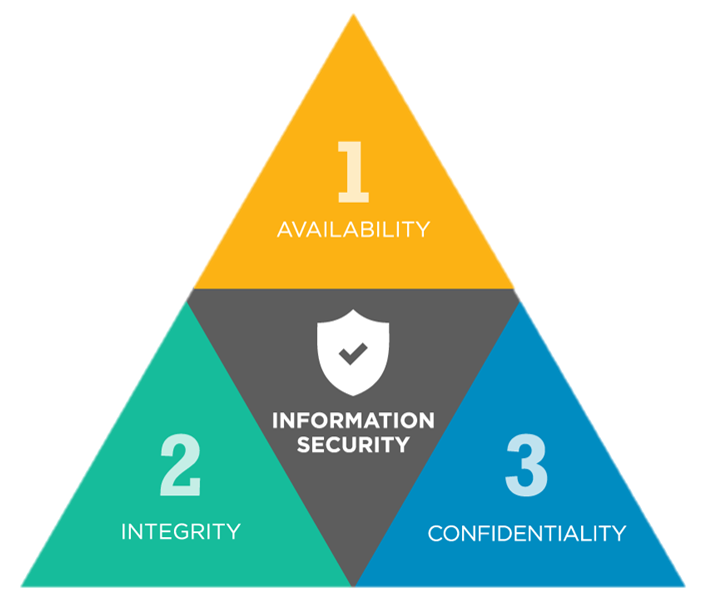
\includegraphics[width=0.5\textwidth]{images/CIA-graph.png}
    \caption{Principles of information security}
    \caption*{\footnotesize\textit{Source: \cite{ibm_principles_of_information_security}}}
    \label{fig:cia-graph}
\end{figure}



\paragraph{Confidentiality} 
Confidentiality ensures that sensitive information is only accessible to authorized users. Techniques such as encryption, user authentication, and access control policies prevent unauthorized data access. While DoS attacks do not typically aim to breach confidentiality directly, successful exploitation may lead to indirect confidentiality violations if attackers cause service misconfigurations or force failovers to insecure states.

\paragraph{Integrity} 
Integrity guarantees that data is accurate and unaltered. It is maintained through cryptographic hash functions, checksums, and digital signatures that validate whether data has been tampered with. During a DoS attack, integrity may be compromised by interrupting legitimate updates or corrupting processes due to system overload.

\paragraph{Availability} 
Availability ensures that services and systems remain accessible to legitimate users at all times. This principle is the primary target of DoS attacks, which flood networks or services with excessive requests, causing slowdowns or complete denial of access. Maintaining availability involves redundancy, load balancing, and proactive mitigation strategies like rate limiting and firewalls.

\subsubsection{Extended Security Principles}

\paragraph{Non-repudiation} 
Non-repudiation guarantees that an entity cannot deny having performed a particular action, such as sending a message or initiating a transaction. This is enforced through digital signatures and secure logging mechanisms. In the context of DoS attacks, non-repudiation helps trace attack origins and supports legal accountability.

\paragraph{Authenticity} 
Authenticity confirms that data, communications, or users are genuine and not forged. Authentication protocols, digital certificates, and cryptographic techniques are used to ensure that data comes from trusted sources. This is crucial for filtering legitimate traffic from spoofed attack traffic in DoS scenarios.

\paragraph{Accountability} 
Accountability ensures that all actions within a system can be traced to responsible users or processes. It involves logging, auditing, and monitoring to track behavior. Accountability is vital for forensic analysis after a DoS attack and for strengthening defenses against future intrusions.

\section{Denial-of-Service (DoS) Attacks}

\paragraph{Introduction} 
Denial-of-Service (DoS) attacks aim to make a system or network resource unavailable to its intended users by overwhelming it with excessive traffic or exploiting protocol-level vulnerabilities. These attacks can disrupt services, degrade performance, or completely shut down access. The most common types include:

\begin{figure}[ht]
    \centering
    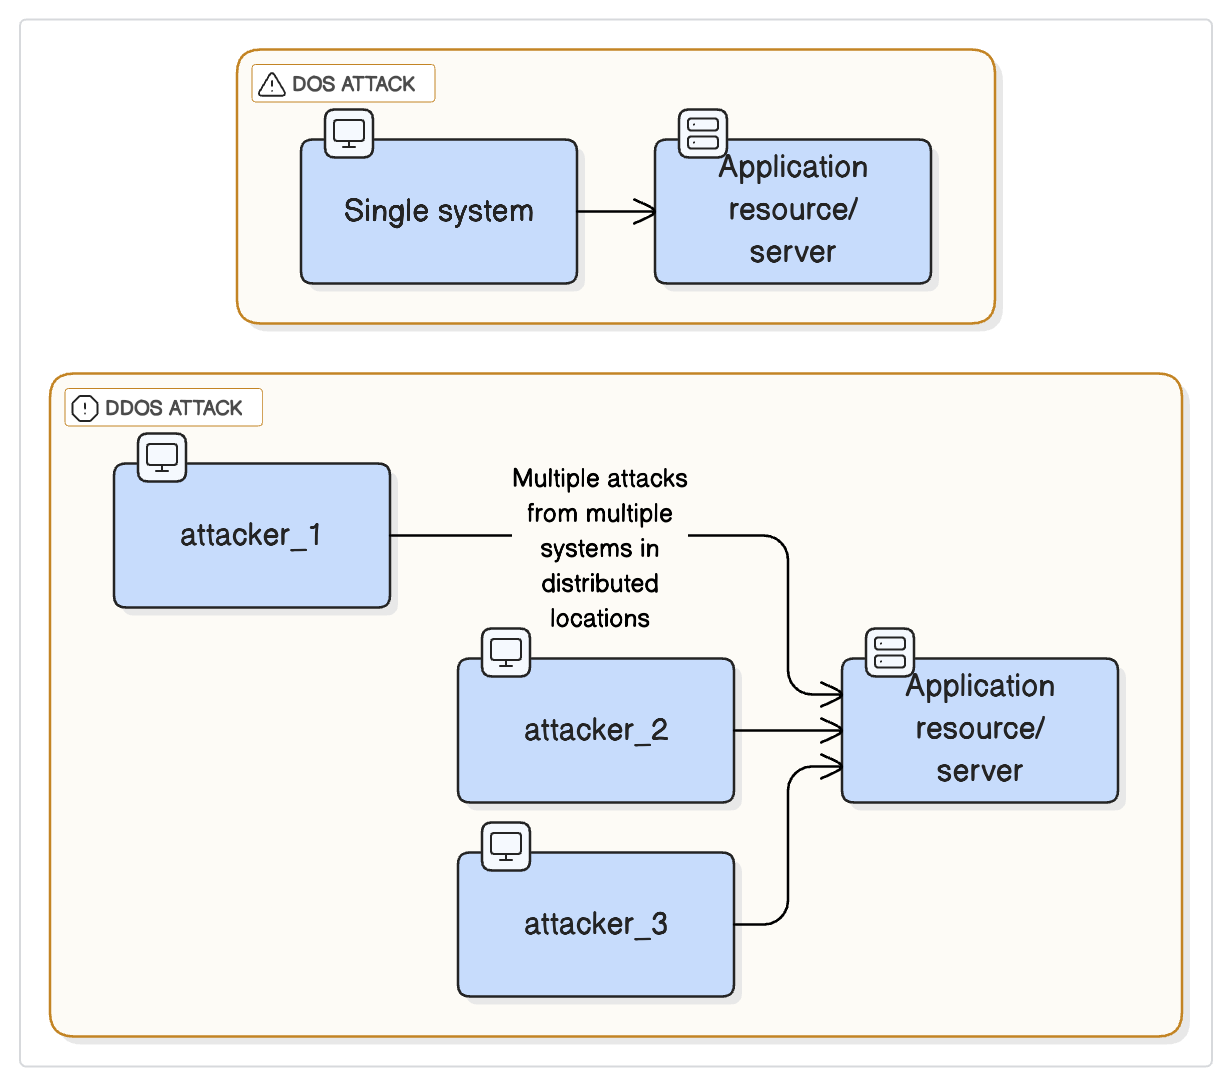
\includegraphics[width=0.8\textwidth]{images/dos-ddos-graph.png}
    \caption{DoS and DDoS Attack Traffic Comparison}
    \vspace{-0.5em}
\end{figure}

\subsection{Volumetric Attacks}
Volumetric attacks aim to saturate a target’s bandwidth by generating an overwhelming amount of traffic. This often involves amplification techniques or high-rate packet floods. Common examples include UDP floods and DNS amplification attacks, which leverage misconfigured servers to multiply traffic directed at the victim~\cite{fidelis_dos}.

In a UDP flood, attackers send large numbers of spoofed UDP packets to random or specific ports, consuming bandwidth and processing power. DNS amplification uses small queries to open resolvers with the victim’s IP address, causing them to return large responses to the victim. 

A notable example is the Mirai botnet, which infected hundreds of thousands of insecure IoT devices to coordinate massive traffic streams toward its targets~\cite{fidelis_dos}. The goal of volumetric attacks is to clog network links (Gbps or Tbps scale), preventing legitimate access.

\subsection{Protocol Attacks}
Protocol attacks exploit weaknesses in Layer 3/4 protocols (network or transport layer) to exhaust server or network resources. Unlike volumetric attacks, they do not require high bandwidth but instead consume stateful resources like connection tables or CPU cycles~\cite{fidelis_dos}.

A classic example is the TCP SYN flood, where attackers send numerous SYN packets without completing the handshake, filling the server’s connection queue~\cite{imperva_dos}. ICMP floods and Ping of Death attacks exploit the Internet Control Message Protocol to crash or freeze systems by sending malformed or excessive traffic.

Other examples include fragmentation attacks (e.g., Teardrop), which send overlapping IP fragments to crash reassembly logic, and ACK/FIN floods that exhaust firewall state tables.

\subsection{Application Layer Attacks}
Application-layer (Layer 7) attacks generate traffic that appears legitimate at the application level but consumes excessive server resources such as CPU, memory, or threads~\cite{fidelis_dos}. These attacks are difficult to detect because they mimic real user behavior.

HTTP GET/POST floods can overwhelm web servers by triggering costly operations. A well-known example is Slowloris, which sends partial HTTP headers slowly to hold open many connections and exhaust the web server’s pool~\cite{netscout_slowloris}. Other examples include RUDY (R-U-Dead-Yet) attacks and HTTP floods targeting dynamic or database-backed content.

\subsection{Distributed Denial-of-Service (DDoS)}
DDoS attacks use multiple compromised machines (botnets) to launch coordinated attacks, making them harder to block and vastly more powerful than single-source DoS attacks~\cite{fidelis_dos}.

Botnets like Mirai leverage IoT devices to simultaneously launch volumetric or protocol-based attacks. Reflective amplification (e.g., using open DNS/NTP servers) further increases traffic impact. Mitigation requires upstream filtering, rate-limiting, and often third-party scrubbing services.

\subsection{Network Traffic Analysis}
Mitigating DoS/DDoS attacks relies on monitoring and anomaly detection. This involves establishing a baseline of normal network behavior and identifying deviations in volume, protocol use, or source IPs~\cite{fidelis_dos, mdpi_dos}.

Anomaly-based intrusion detection systems (IDS) can flag unusual spikes, connection patterns, or TCP flag anomalies. Signature-based systems match known attack patterns. Flow analysis tools (e.g., NetFlow, sFlow) help detect irregular byte/packet rates or unusual source-destination pairs.

Advanced methods include machine learning to classify deviations. Once detected, defenses such as rate limiting, traffic shaping, or redirection to mitigation services are employed to maintain availability.


% \paragraph{Introduction} 
% Denial-of-Service (DoS) attacks aim to make a system or network resource unavailable to its intended users by overwhelming it with excessive traffic or exploiting protocol-level vulnerabilities. These attacks can disrupt services, degrade performance, or completely shut down access. The most common types include:

% \begin{figure}[ht]
%     \centering
%     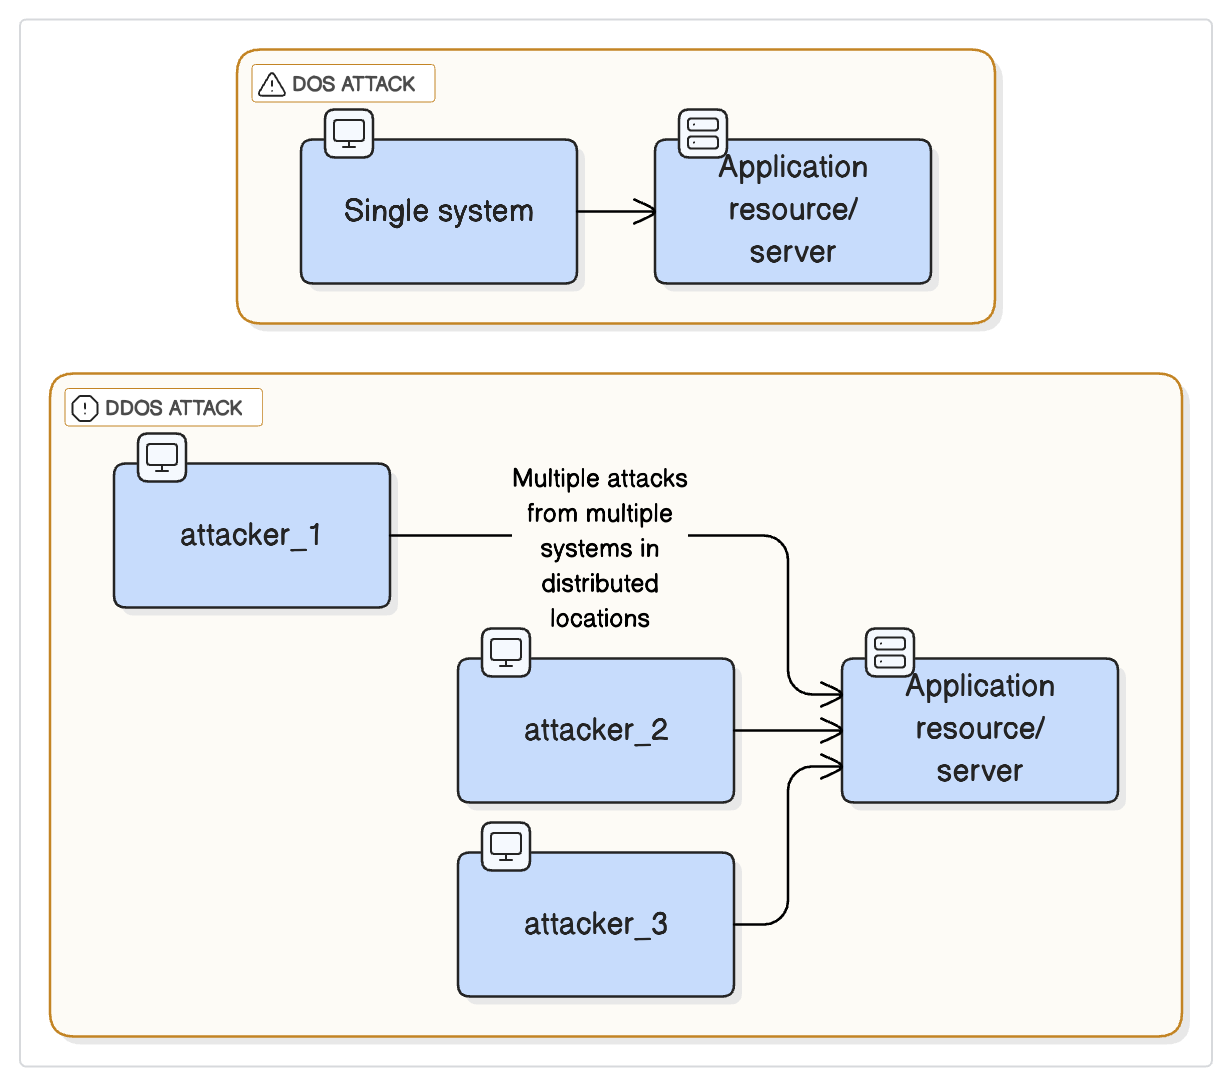
\includegraphics[width=0.5\textwidth]{images/dos-ddos-graph.png} 
%     \caption{DoS and DDoS Attack Traffic Comparison}
%     \vspace{-0.5em} % Optional: reduces space between caption and following text
% \end{figure}


% \section{Denial-of-Service (DoS) Attacks} \subsection{Volumetric Attacks}
% Volumetric attacks aim to saturate a target’s bandwidth by generating an overwhelming amount of traffic. This often involves exploiting amplification techniques or high-rate packet floods. Common examples include UDP floods and DNS amplification attacks, which leverage misconfigured servers to multiply the traffic volume directed at the victim
% fidelissecurity.com
% . In a UDP flood, for instance, an attacker sends vast numbers of UDP packets (often with spoofed source addresses) to random or specific ports on the target, forcing the target to process or drop them and thereby consuming bandwidth. In DNS amplification, the attacker sends small DNS queries to open resolvers with the victim’s IP as the source address; each resolver then returns a much larger response to the victim, effectively amplifying the traffic volume. The Mirai botnet is a notable example of a volumetric attack in action: it infected hundreds of thousands of insecure IoT devices and coordinated them to generate massive traffic streams toward its targets
% fidelissecurity.com
% . The ultimate goal of volumetric attacks is to clog the network links (measured in Gbps or Tbps) so that legitimate traffic cannot reach the target. \subsection{Protocol Attacks}
% Protocol attacks exploit weaknesses in network or transport layer protocols (OSI Layer 3/4) to exhaust server or network equipment resources. Unlike volumetric attacks that focus on bandwidth, protocol attacks aim to consume connection state tables or CPU cycles by misusing fundamental protocol mechanisms
% fidelissecurity.com
% . A classic example is the TCP SYN flood: the attacker sends a rapid stream of TCP SYN packets to initiate connections but never completes the three-way handshake. Each half-open connection consumes memory and processing power on the server, so with enough such requests the server’s backlog queue fills up and it can no longer accept new legitimate connections
% imperva.com
% . Similarly, ICMP-based attacks exploit the Internet Control Message Protocol: a Ping flood (ICMP flood) can overwhelm a target by sending large volumes of ICMP echo requests, while the Ping of Death sends malformed or oversized ICMP packets (larger than the 65,535-byte IPv4 limit) that can crash or freeze vulnerable systems
% imperva.com
% . Other protocol-layer examples include packet fragmentation attacks (e.g.\ the Teardrop attack, which sends overlapping IP fragments to disrupt reassembly) and ACK/FIN floods, all of which aim to tie up connection tables or processing resources on routers and servers. These attacks often do not require as much raw bandwidth as volumetric floods, but they exploit the target’s protocol handling to disrupt service. \subsection{Application Layer Attacks}
% Application-layer (Layer 7) attacks are characterized by generating traffic that appears to be legitimate or normal at the application level, thereby exhausting server-side resources such as CPU, memory, or thread pools. Because these attacks mimic regular user behavior (for example, HTTP requests or API calls), they can be harder to distinguish from genuine traffic. For instance, an HTTP GET/POST flood might involve hundreds of thousands of seemingly valid requests to a web server or API endpoint, causing the server to spawn processes or threads until it is overwhelmed. A well-known application-layer attack is Slowloris: it sends partial HTTP requests to a web server and never completes them, keeping the connections open indefinitely and consuming the server’s connection pool
% netscout.com
% . Slowloris effectively slows down the server by forcing it to maintain a large number of half-open HTTP connections, with minimal bandwidth required by the attacker. Other examples include “RUDY” (R-U-Dead-Yet) attacks, which continually send small pieces of an HTTP POST request to tie up server resources, and HTTP GET floods targeting expensive dynamic pages or database-backed resources. In general, application-layer attacks target the web server or application functions (e.g.\ API endpoints or login pages) directly
% fidelissecurity.com
% . Because the traffic can look valid (for example, proper HTTP syntax or valid query parameters), application-layer attacks often require careful behavioral analysis or specialized filters to detect. \subsection{Distributed Denial-of-Service (DDoS)}
% A Distributed Denial-of-Service (DDoS) attack uses multiple compromised machines (often thousands of bots forming a botnet) to launch a coordinated assault on a target. By originating traffic from many different IP addresses and locations, a DDoS attack can generate a vastly higher volume of traffic than a single-host DoS, and it is much harder to block simply by filtering individual IPs
% fidelissecurity.com
% . DDoS campaigns often combine vectors: for example, a multi-vector attack might include simultaneous UDP or TCP floods along with HTTP floods. Commonly, attackers use botnets of compromised devices (such as IoT devices infected by Mirai or hijacked PCs) to send traffic in unison. Reflective amplification attacks are also typical DDoS techniques: the attacker sends requests (with the victim’s spoofed IP) to large groups of open DNS or NTP servers, which in turn send amplified responses to the victim, effectively multiplying the traffic from many sources. The distributed and high-scale nature of DDoS makes mitigation challenging, since simply blocking one source or one protocol is usually insufficient. In practice, DDoS defenses often rely on upstream filtering, specialized scrubbing services, and the ability to absorb or redistribute very high traffic volumes
% fidelissecurity.com
% . \subsection{Network Traffic Analysis}
% Detecting and mitigating DoS/DDoS attacks requires continuous monitoring of network traffic to identify deviations from normal patterns. A key approach is to establish a baseline of typical traffic (volume, packet rates, protocols, source distributions) and then use anomaly detection to flag unusual deviations. For example, a sudden, sustained spike in traffic volume or connection attempts (far above normal business hours levels) is a classic indicator of a volumetric or protocol-layer attack
% fidelissecurity.com
% . An anomaly-based intrusion detection system (IDS) can alert when traffic exceeds expected thresholds or when the profile of traffic (such as packet sizes, TCP flag patterns, or new IP addresses) changes markedly
% mdpi.com
% . Signature-based detection can also be used: known patterns (e.g.\ large numbers of SYN packets without ACK, or unusual payload characteristics) are matched against traffic to detect certain types of DoS. Network flow analysis (using NetFlow, sFlow or similar records) is another important tool: by aggregating traffic statistics, analysts can detect irregular surges in bytes or packets per second, or anomalous flows such as many sources contacting a single destination. More advanced systems apply statistical and machine learning methods to continuously learn normal behavior and classify deviations as malicious. In practice, effective DDoS detection often combines multiple techniques – for example, automated tools may raise an alarm when both the volume of traffic and the rate of new TCP connections simultaneously spike
% mdpi.com
% fidelissecurity.com
% . Once an attack is detected, defenses such as traffic shaping, rate limiting, or rerouting through mitigation services can be applied to preserve service availability.

% \paragraph{Volumetric Attacks} 
% These attacks consume all available bandwidth by sending massive amounts of traffic, such as in UDP floods or ICMP amplification attacks. Their goal is to exhaust network capacity, making it impossible for legitimate traffic to pass through.

% \paragraph{Protocol Attacks} 
% Protocol-based DoS attacks exploit weaknesses in layer 3 and 4 of the OSI model. For example, a SYN flood abuses the TCP handshake by initiating numerous incomplete connections, which fill up server resources and prevent new connections from being established.

% \paragraph{Application Layer Attacks} 
% These target the application layer (Layer 7) by mimicking legitimate user behavior to exhaust server-side resources. Attacks like Slowloris maintain open HTTP connections for extended periods, gradually consuming server threads without sending complete requests.

% \paragraph{Distributed Denial of Service (DDoS)} 
% DDoS attacks are coordinated from multiple compromised systems, often forming a botnet. These attacks can be volumetric, protocol-based, or application-layer focused, but their distributed nature makes them harder to mitigate due to the scale and diversity of sources.

% \subsection{Network Traffic Analysis}
% To effectively detect DoS attacks, it is necessary to monitor and analyze network traffic for deviations from normal behavior.


% \subsubsection{Baseline Metrics}
% \begin{itemize}
%     \item \textbf{Packets per Second (PPS):} Measures the rate of incoming or outgoing packets.
%     \item \textbf{Bandwidth Consumption:} Refers to the typical volume of data transferred.
%     \item \textbf{Connection Rates:} Tracks the number of new connections established over time.
%     \item \textbf{Protocol Distribution:} Observes the usual mix of network protocols like TCP, UDP, and ICMP.
%     \item \textbf{Time-of-Day Patterns:} Identifies regular traffic cycles, such as business hour spikes.
% \end{itemize}

% \subsubsection{Types of Anomalies}
% \begin{itemize}
%     \item \textbf{Volume Anomalies:} Sudden increases in traffic volume, which may indicate floods or amplification attacks.
%     \item \textbf{Pattern Anomalies:} Changes in traffic behavior, such as irregular packet intervals or source IP variation.
%     \item \textbf{Content Anomalies:} Malformed packets or protocol violations that suggest tampered or malicious payloads.
% \end{itemize}

% \subsubsection{Traffic Analysis Techniques}
% \begin{itemize}
%     \item \textbf{Statistical Profiling:} Identifies deviations from normal traffic metrics.
%     \item \textbf{Time-Series Analysis:} Detects patterns and trends over time.
%     \item \textbf{Correlation Analysis:} Links multiple traffic attributes to identify coordinated attacks.
%     \item \textbf{Entropy Measurement:} Evaluates randomness in traffic data to detect anomalies.
% \end{itemize}


\section{Intrusion Detection Systems (IDS)}

An \textbf{Intrusion Detection System (IDS)} is a cybersecurity solution designed to monitor network or system activities for malicious actions or policy violations. Upon detecting such activities, the IDS typically alerts system administrators or integrates with centralized security tools like Security Information and Event Management (SIEM) systems to facilitate a coordinated response \cite{ibm_ids}.

% \subsection{Types of IDS}

% IDS solutions can be categorized based on their monitoring focus:

% \begin{itemize}
%     \item \textbf{Network-based IDS (NIDS)}: Monitors network traffic for suspicious activity.
%     \item \textbf{Host-based IDS (HIDS)}: Monitors individual devices or hosts for signs of malicious behavior \cite{wikipedia_ids}.
% \end{itemize}

% \subsection{Detection Methods}

% Detection methods employed by IDS include:

% \begin{itemize}
%     \item \textbf{Signature-based Detection}: Identifies known threats by comparing patterns against a database of attack signatures.
%     \item \textbf{Anomaly-based Detection}: Detects deviations from established normal behavior, potentially identifying unknown threats \cite{fortinet_ids}.
% \end{itemize}

% \subsection{Functionality}

% While traditional IDS solutions are passive—monitoring and alerting without taking direct action—some modern systems incorporate proactive measures. These advanced IDS can respond to detected threats by, for example, blocking malicious traffic or isolating affected systems, thereby functioning similarly to Intrusion Prevention Systems (IPS) \cite{techtarget_ids}.

% Incorporating an IDS into an organization's cybersecurity infrastructure enhances its ability to detect and respond to potential threats, thereby safeguarding sensitive data and maintaining system integrity.





% \section{Intrusion Detection Systems (IDS)}

% An Intrusion Detection System (IDS) is a security solution—either software, hardware, or a combination—that continuously monitors the activity of a computer network or individual hosts in order to spot signs of malicious behavior, policy violations, or other unauthorized actions. By collecting "raw" data from packet captures, system logs, file-access events or operating-system calls, an IDS uses a set of predefined rules (signatures of known attacks) and/or statistical models of normal behavior (anomaly detection) to flag suspicious patterns. When such patterns are detected, the IDS generates alerts for security analysts or—if so configured—triggers automated responses, such as blocking malicious IP addresses or quarantining affected machines. In this way, an IDS serves as an early‐warning system that helps organizations identify and respond to intrusions before they escalate into full-blown breaches.

\subsection{IDS Architecture}

\begin{figure}[H]
    \begin{minipage}{\textwidth}
        \hspace*{-0.05\linewidth}
        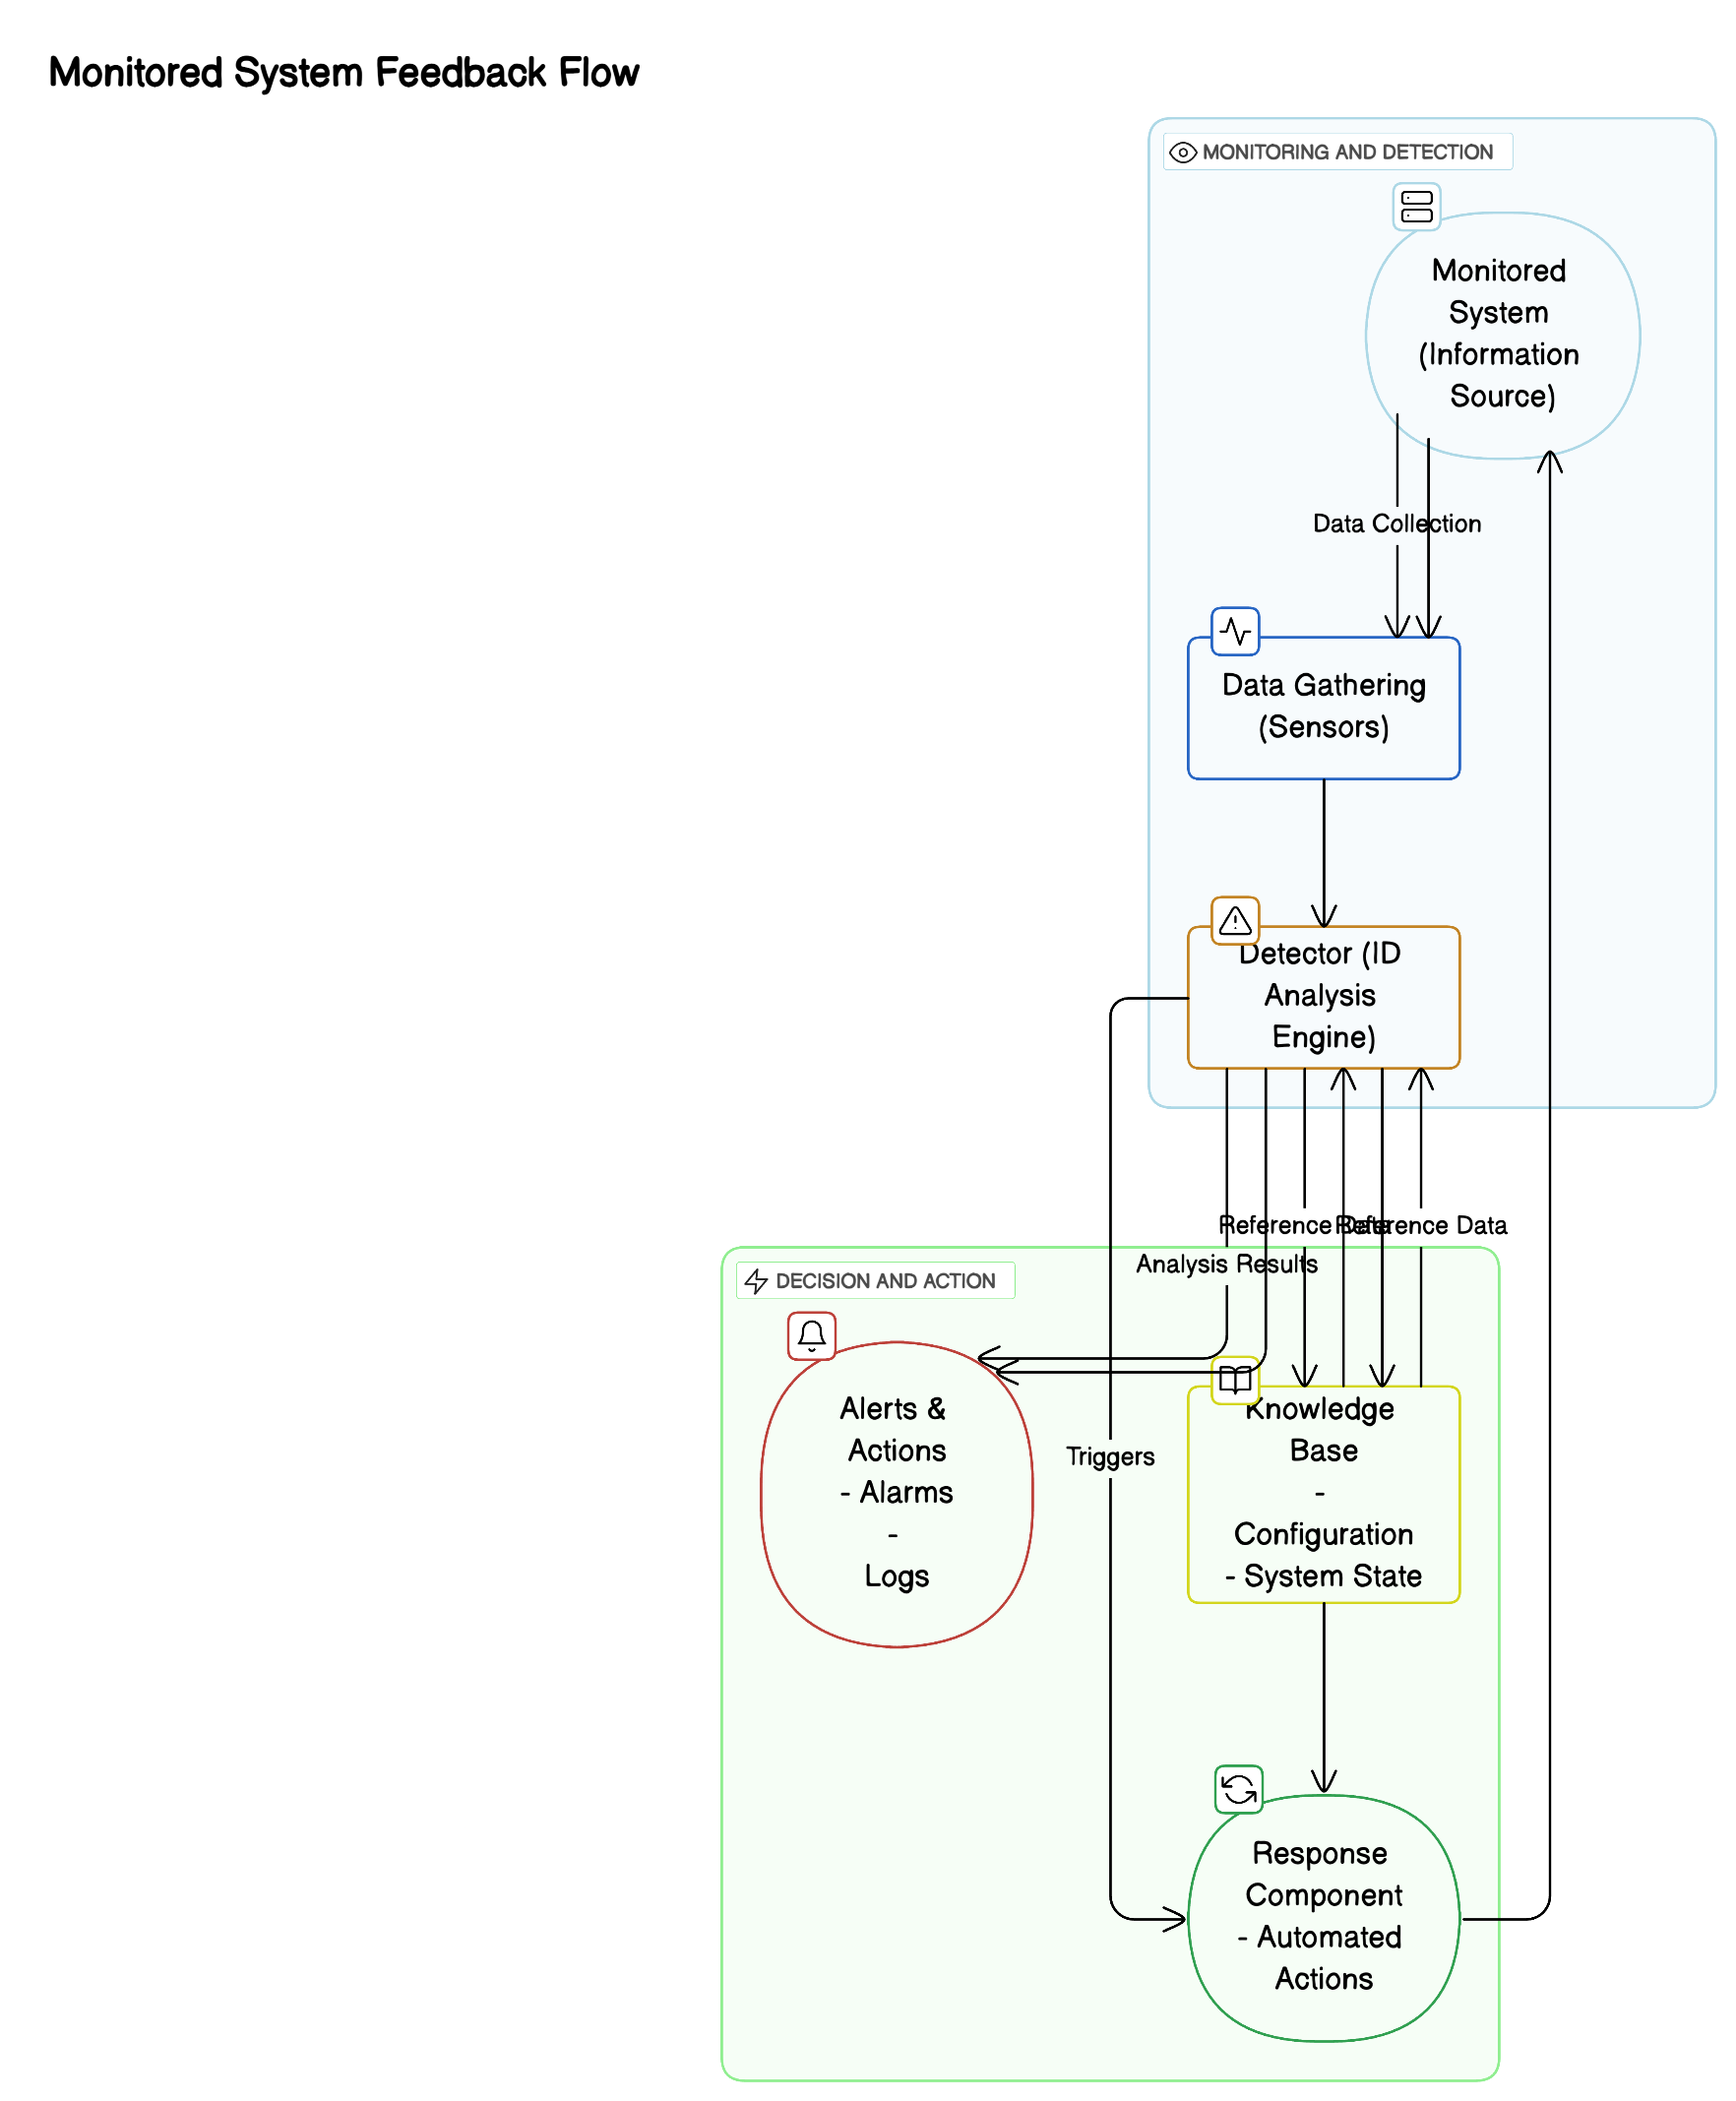
\includegraphics[width=0.8\textwidth]{images/ids-arch-diagram.png}
        \caption{Network-based Intrusion Detection System (NIDS) Architecture}
        \label{fig:nids-architecture}
    \end{minipage}
\end{figure}




Modern IDS platforms implement modular architectures with several key components:

\begin{itemize}
\item \textbf{Sensors:}
are the front line of an IDS, deployed at strategic network chokepoints—such as mirror (SPAN) ports, network taps, or virtual interfaces in cloud environments—to collect raw traffic data. They capture full packet streams, flow records, or application logs and often include built-in filters or sampling mechanisms to reduce noise in high-volume settings. By pre-processing and forwarding only relevant events, sensors ensure the IDS receives a representative yet manageable dataset, enabling visibility into lateral movement, data exfiltration, and denial-of-service attempts without overwhelming the analysis layer.

\item \textbf{Analysis Engines:}
Analysis Engines form the IDS's "brain," taking the sensor-collected data and applying a mixture of rule-based and intelligent techniques to detect threats. Traditional pattern-matching engines compare payloads against known attack signatures, while statistical or machine-learning analyzers establish behavioral baselines and flag deviations. Protocol analyzers dive deep into application-level conversations—HTTP, DNS, SMB, etc.—to spot malformed requests or anomalous sequences. By correlating events across multiple sensors and data sources, the engine can piece together multi-stage attacks (e.g., a scan followed by an exploit) and prioritize alerts based on risk.

\item \textbf{Knowledge Base:}
The Knowledge Base underpins all detection logic by maintaining up-to-date signatures, behavioral profiles, and historical datasets. Signature databases are refreshed with the latest threat intelligence feeds, while anomaly detectors continuously refine their statistical models using both live traffic and feedback on past alerts. In more advanced platforms, machine-learning feedback loops incorporate security analyst verdicts—true positive, false positive—to retrain the system, improving accuracy over time. This shared repository ensures that the IDS can recognize both known exploits and subtle shifts in normal network behavior.

\item \textbf{Response Systems:}
Response Systems close the loop between detection and defense. Once the analysis engine assigns a confidence score to an event, the response component generates alerts—pushing them into dashboards, SIEMs, or ticketing systems—and, where policies allow, triggers automated countermeasures. High-confidence detections might invoke firewall rule updates, IP blacklists, or host quarantines, while lower-confidence events are routed to alert managers for human review. Integrated visualization tools help security teams triage incidents rapidly, and orchestration connectors enable the IDS to participate in broader security workflows, ensuring a coordinated, efficient reaction—especially critical when facing large-scale DoS or DDoS onslaughts.
\end{itemize}

For DOS attack detection, these components must operate with high efficiency and scale to process enormous traffic volumes during attack scenarios.

\subsection{IDS Types and Functionality}

Intrusion Detection Systems serve as the primary monitoring and detection layer for network security threats, including DOS attacks:

\begin{itemize}
\item \textbf{Network-based IDS (NIDS):}
A Network-based Intrusion Detection System (NIDS) is a monitoring solution placed at key junctions within a network—often on a mirrored switch port or network tap—where it passively captures and inspects all passing traffic. Unlike host‐based agents, a NIDS doesn't rely on software installed on individual machines; instead, it reconstructs network sessions and analyzes packet headers and payloads in real time. It uses signature‐based detection (comparing packets against a database of known attack patterns) and anomaly‐based detection (profiling normal traffic volumes, protocols, and behavioral baselines) to spot suspicious or malicious activity—such as port scans, denial-of-service floods, SQL injection attempts, or data exfiltration. When the NIDS flags a potential intrusion, it generates an alert that can be logged centrally, forwarded to a Security Information and Event Management (SIEM) system, or used to trigger automated defenses (e.g., instructing a firewall to block the offending IP). Because it sees all traffic crossing its monitored segment, a properly tuned NIDS provides broad visibility into attacker reconnaissance and network‐level exploits—though it can be blind to encrypted payloads unless integrated with SSL/TLS decryption, and it may generate false positives if thresholds or signatures aren't carefully calibrated. By complementing host‐based sensors and other controls, a NIDS forms a crucial layer in a network's defense-in-depth strategy.

  \begin{center}
    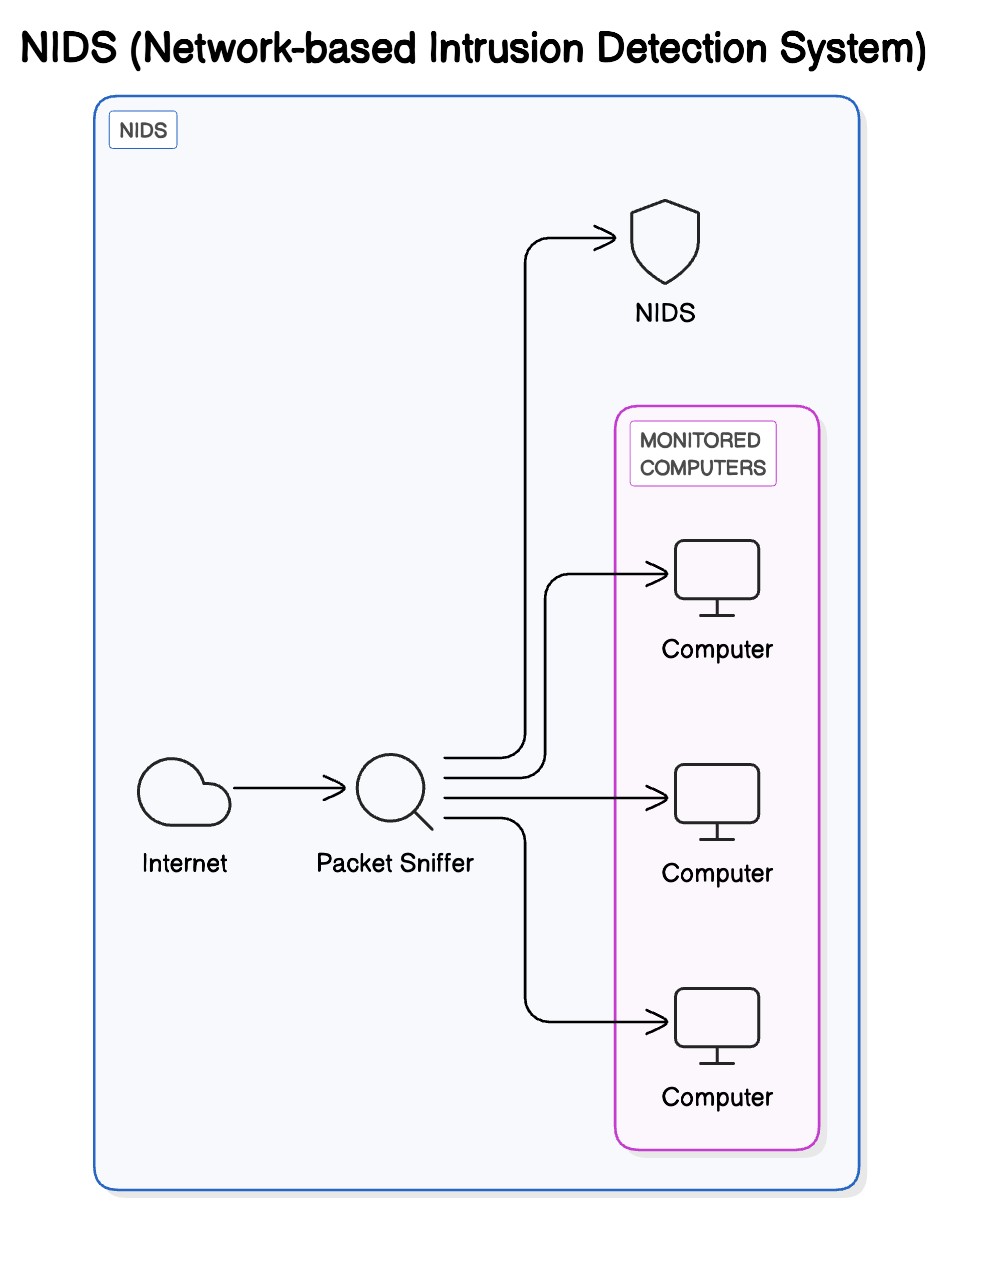
\includegraphics[width=0.8\textwidth]{images/nids-diagram.png} \\
    \textit{Figure: Network-based Intrusion Detection System (NIDS) Architecture}
  \end{center}
\item \textbf{Host-based IDS (HIDS):}
A Host-based Intrusion Detection System (HIDS) operates at the level of individual endpoints or servers, offering deep visibility into system-specific activities. Instead of analyzing network traffic, HIDS monitors internal events such as system calls, file integrity changes, registry modifications, user logins, and local log files. This allows it to detect unauthorized alterations, privilege escalations, malware activity, and localized impacts of denial-of-service (DoS) attacks that may not be evident from a network perspective. By focusing on what happens inside the host, HIDS provides rich contextual information—such as which process triggered a suspicious action or which user account was involved—which is crucial for forensic analysis and containment. However, its scope is inherently limited to the device it protects, offering little visibility into lateral movement or network-wide attack patterns. Common examples of HIDS tools include OSSEC, Tripwire, and Wazuh.
  \begin{center}
    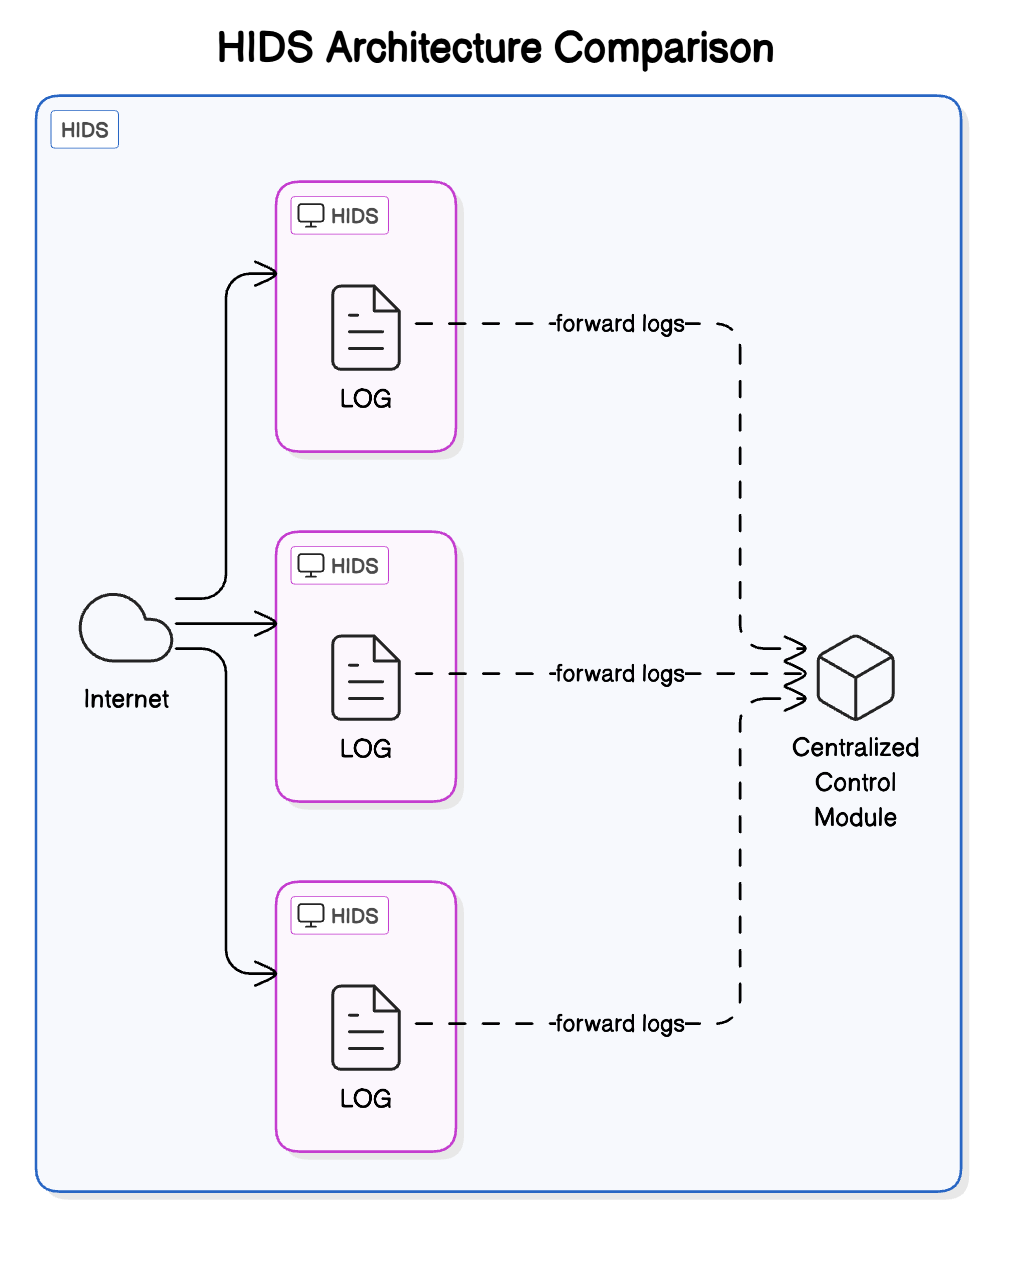
\includegraphics[width=0.8\textwidth]{images/hids-diagram.png} \\
    \textit{Figure: Network-based Intrusion Detection System (NIDS) Architecture}
  \end{center}
\item \textbf{Detection Methodologies:}
  \begin{itemize}
  \item \textbf{Signature-based:} Matches observed traffic against known attack patterns (signatures)
    \begin{itemize}
    \item Highly effective for known attacks with clear signatures
    \item Requires regular signature updates
    \item Ineffective against zero-day or modified attacks
    \item Examples: SYN flood patterns, known botnet command signatures
    \end{itemize}
    
  \item \textbf{Anomaly-based:} Establishes baselines of normal behavior and flags significant deviations
    \begin{itemize}
    \item Can detect previously unknown attack vectors
    \item Requires training period to establish accurate baselines
    \item Typically generates more false positives than signature-based systems
    \item Examples: Traffic volume spikes, unusual protocol distributions
    \end{itemize}
    
  \item \textbf{Hybrid Systems:} Combine signature and anomaly detection approaches
    \begin{itemize}
    \item Leverage strengths of both methodologies
    \item Use signatures for known threats and anomaly detection for novel attacks
    \item Implement weighted alert systems for confidence scoring
    \item Reduce false positives through correlation of multiple detection methods
    \end{itemize}
  \end{itemize}
\end{itemize}

Limitations of Traditional IDS for DOS attack detection include:
\begin{itemize}
\item Difficulty processing high-volume traffic during attacks
\item Challenges distinguishing flash crowds from attacks
\item Limited adaptation to evolving attack techniques
\item High false-positive rates with anomaly detection
\item Resource consumption during high-traffic periods
\end{itemize}

These limitations necessitate AI-driven approaches like reinforcement learning that can adapt to evolving threat landscapes.

\section{Classification in Security Contexts}

\subsection{Classification Paradigms}

Classification forms the foundation of automated threat detection, organizing network traffic into categories for analysis and response:

\textbf{Binary Classification:} The simplest approach for distinguishing between normal and attack traffic. This method provides clear decision boundaries for basic filtering with low granularity but high processing efficiency. It is essential for initial traffic triage during high-volume attacks, offering straightforward pass/block decisions and benign/malicious categorization.

\textbf{Multi-class Classification:} A more sophisticated approach that distinguishes between multiple attack types, enabling targeted responses for specific threats. While requiring more complex models and training data, this method supports detailed attack attribution and can differentiate between various attack vectors such as SYN floods, HTTP floods, and DNS amplification attacks.

\textbf{Hierarchical Classification:} An organized approach that structures threats in a tree-like format, enabling progressive refinement of classifications. This method balances processing efficiency with detection detail and supports multi-stage detection pipelines. For example, traffic can be progressively classified as: Traffic → Attack → DOS → Protocol-based → SYN Flood.

\textbf{Multi-label Classification:} An advanced approach that assigns multiple categories to a single traffic flow, recognizing attacks with multiple characteristics. This method identifies complex attack campaigns and supports sophisticated response orchestration. For instance, traffic can be simultaneously classified as "volumetric," "distributed," and "amplification."
% \begin{itemize}
% \item \textbf{Binary Classification:}
%   \begin{itemize}
%   \item Simplest approach: Normal vs. attack traffic
%   \item Clear decision boundaries for basic filtering
%   \item Low granularity but high processing efficiency
%   \item Essential for initial traffic triage during high-volume attacks
%   \item Examples: Pass/block decisions, benign/malicious categorization
%   \end{itemize}
  
% \item \textbf{Multi-class Classification:}
%   \begin{itemize}
%   \item Distinguishes between multiple attack types
%   \item Enables targeted responses for specific threats
%   \item Requires more complex models and training data
%   \item Supports detailed attack attribution
%   \item Examples: Differentiating SYN floods, HTTP floods, DNS amplification attacks
%   \end{itemize}
  
% \item \textbf{Hierarchical Classification:}
%   \begin{itemize}
%   \item Organizes threats in a tree-like structure
%   \item Enables progressive refinement of classifications
%   \item Balances processing efficiency with detection detail
%   \item Supports multi-stage detection pipelines
%   \item Example: Traffic → Attack → DOS → Protocol-based → SYN Flood
%   \end{itemize}
  
% \item \textbf{Multi-label Classification:}
%   \begin{itemize}
%   \item Assigns multiple categories to a single traffic flow
%   \item Recognizes attacks with multiple characteristics
%   \item Identifies complex attack campaigns
%   \item Supports sophisticated response orchestration
%   \item Example: Traffic simultaneously classified as "volumetric," "distributed," and "amplification"
%   \end{itemize}
% \end{itemize}


Classification outcomes drive security responses, determining whether traffic should be allowed, throttled, redirected, or blocked entirely.

\section*{What is Machine Learning?}

Machine learning (ML) is a branch of artificial intelligence (AI) focused on enabling computers and machines to imitate the way that humans learn, to perform tasks autonomously, and to improve their performance and accuracy through experience and exposure to more data.

According to UC Berkeley, the learning system of a machine learning algorithm can be broken down into three main parts:

\begin{enumerate}
    \item \textbf{A Decision Process:} In general, machine learning algorithms are used to make a prediction or classification. Based on some input data, which can be labeled or unlabeled, the algorithm produces an estimate about a pattern in the data.
    
    \item \textbf{An Error Function:} An error function evaluates the prediction of the model. If there are known examples, an error function can make a comparison to assess the accuracy of the model.
    
    \item \textbf{A Model Optimization Process:} If the model can fit better to the data points in the training set, then weights are adjusted to reduce the discrepancy between the known example and the model estimate. The algorithm repeats this iterative ``evaluate and optimize'' process, updating weights autonomously until a threshold of accuracy has been met.
\end{enumerate}

\noindent\textbf{Source:} \href{https://www.ibm.com/think/topics/machine-learning}{https://www.ibm.com/think/topics/machine-learning}

\subsection{Machine Learning Techniques}

Modern security systems leverage diverse machine learning approaches for traffic classification:


\section*{Supervised Learning}

Supervised learning involves training on labeled datasets where the "ground truth" classifications of attacks are already known. This approach allows models to learn from past data and make accurate predictions on new, unseen inputs. Common algorithms used in supervised learning include Random Forests, which are ensembles of decision trees that offer robust classification; Support Vector Machines (SVM), which are effective at identifying decision boundaries between different types of network traffic; Neural Networks, including multi-layer perceptrons and deep learning architectures capable of recognizing complex patterns; and Gradient Boosting methods like XGBoost, which are known for their high-performance classification capabilities. Supervised learning is especially useful in scenarios such as detecting known attacks using labeled training data, identifying specific types of attacks, analyzing the importance of different features, and deploying models in production environments where minimizing false positives is crucial.

\section*{Unsupervised Learning}

Unsupervised learning focuses on uncovering patterns and structures within data that has not been labeled. This approach is especially useful when dealing with vast amounts of network traffic where manual labeling is impractical or impossible. Techniques commonly used in unsupervised learning include clustering methods such as \textit{k}-means and DBSCAN, which group similar traffic patterns together based on statistical similarity. Anomaly detection methods like Isolation Forest and One-Class SVM are effective for identifying outliers that may indicate potential security threats. Dimensionality reduction techniques such as Principal Component Analysis (PCA) and t-Distributed Stochastic Neighbor Embedding (t-SNE) are used to simplify complex traffic data, making it easier to analyze. Autoencoders, a type of neural network, learn representations of normal traffic behavior and can highlight anomalies when deviations occur. Unsupervised learning is particularly valuable for identifying novel attack patterns, establishing baselines for normal behavior, detecting zero-day attacks, and categorizing traffic without the need for prior labeling.

\section*{Semi-Supervised Learning}

Semi-supervised learning bridges the gap between supervised and unsupervised approaches by combining a small amount of labeled data with a much larger pool of unlabeled data. This method reduces the need for extensive manual labeling while still achieving reasonable accuracy in classification. It is especially beneficial in cybersecurity contexts where labeled attack data may be scarce, but large amounts of raw traffic data are available. Techniques in this category include self-training classifiers, where the model iteratively labels new data based on its predictions, and label propagation methods, which spread label information across a data graph based on similarity. Semi-supervised learning is particularly valuable in dynamic and evolving threat landscapes, where continuous adaptation to new types of attacks is required without exhaustive annotation efforts.

\vspace{1em}
These approaches also form the foundation for reinforcement learning systems, which build upon the outcomes of classification tasks to develop and refine optimal security policies.

\chapter{Reinforcement Learning Applications: A Comprehensive Guide}

\section{Introduction to the Reinforcement Learning Approach}

Reinforcement Learning (RL) is a branch of machine learning that focuses on how agents can learn to make decisions through trial and error to maximize cumulative rewards. Unlike supervised learning, where models learn from labeled data, RL involves learning optimal behaviors through interactions with an environment, receiving feedback in the form of rewards or penalties based on actions taken. This approach enables agents to discover strategies that yield the highest long-term benefits, making RL particularly effective for tasks involving sequential decision-making, such as robotics, game playing, and autonomous systems.
Reinforcement Learning provides several key advantages over traditional DoS detection approaches:

\noindent\textbf{Source:} Adapted from GeeksforGeeks: What is Reinforcement Learning
\section{Introduction to Deep Q-Learning}

Deep Q-Learning is a powerful extension of the traditional Q-Learning algorithm that leverages deep neural networks to approximate the Q-value function. In standard Q-Learning, an agent maintains a Q-table that maps state-action pairs to expected future rewards. However, this becomes impractical for environments with large or continuous state spaces. Deep Q-Learning addresses this limitation by using a deep neural network, known as a Q-network, to estimate Q-values directly from raw input states.

In reinforcement learning, the agent interacts with the environment in discrete time steps. At each step $t$, the agent observes a state $s_t$, selects an action $a_t$, receives a reward $r_t$, and transitions to a new state $s_{t+1}$. The goal is to learn a policy $\pi$ that maximizes the expected cumulative reward over time.

The Q-value function $Q(s, a)$ represents the expected return of taking action $a$ in state $s$ and following the policy thereafter. In Deep Q-Learning, the Q-network is trained to minimize the difference between the predicted Q-value and the target Q-value, which is computed using the Bellman equation:

\begin{equation}
Q(s\_t, a\_t) = r\_t + \gamma \max\_{a'} Q(s\_{t+1}, a'; \theta^-)
\end{equation}

Here, $\gamma$ is the discount factor, $\theta$ are the parameters of the current Q-network, and $\theta^-$ are the parameters of a target network that is periodically updated to stabilize training.

To improve learning stability and efficiency, Deep Q-Learning introduces two key techniques:
\begin{itemize}
\item \textbf{Experience Replay:} Stores past experiences in a replay buffer and samples mini-batches randomly during training to break correlations between consecutive samples.
\item \textbf{Target Network:} Uses a separate, periodically updated target network to compute the target Q-values, reducing oscillations and divergence.
\end{itemize}

Deep Q-Learning has been successfully applied to various complex decision-making tasks, such as playing Atari games directly from raw pixels, demonstrating its potential in handling high-dimensional input spaces.


 \begin{center}
    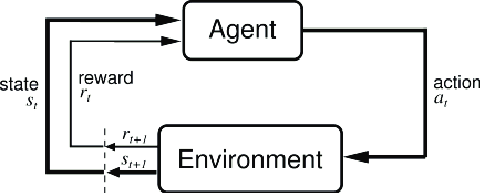
\includegraphics[width=0.8\textwidth]{images/rl-diagram.png} \\
    \textit{Figure: Basic Components of Reinforcement Learning}
  \end{center}

\section{Environment Modeling for DoS Detection}

The foundation of any RL application is a well-designed environment that accurately represents the problem domain. For DoS detection, this environment must model network traffic patterns and attack scenarios in a way that enables effective learning.

\subsection{State Space Design}

The state space in a reinforcement learning (RL) framework for Denial-of-Service (DoS) detection encodes the essential characteristics of network traffic that the agent uses to make decisions. A well-designed state space should reflect a comprehensive yet efficient representation of the network environment, enabling the RL agent to distinguish between normal and malicious activity. This design typically integrates four categories of features: traffic volume metrics, statistical distribution properties, temporal behavior indicators, and content-based descriptors. Each category offers a unique perspective on the nature of the traffic, contributing to a robust and informative state representation.

Traffic volume features quantify the scale and frequency of network activity. These include metrics such as packets per second, bytes per second, flow initiation rates, and the number of concurrent connections. These indicators are particularly useful for detecting volumetric DoS attacks, which are characterized by sudden spikes in traffic volume designed to overwhelm network resources. By monitoring these patterns, the RL agent can quickly recognize and react to abnormal surges in activity.

Statistical distribution features capture how traffic attributes are spread across various dimensions. Entropy values of source and destination IP addresses, protocol usage percentages, port distributions, and packet size variation are key indicators in this category. These features help identify anomalies that are not necessarily reflected in overall traffic volume but manifest as irregularities in distribution patterns, such as a high concentration of traffic targeting a specific port or originating from a narrow set of addresses.

Temporal pattern features provide insight into the evolution of traffic over time. By analyzing short-term trends, comparing current behavior to historical baselines, or evaluating periodicity, the agent can detect subtle or persistent attack patterns. Features such as time-of-day normalization or trend analysis allow the RL agent to differentiate between expected daily fluctuations and genuinely suspicious behavior, such as traffic bursts that align with known attack schedules.

Content-based features delve into the specifics of packet content and header information. This includes identifying protocol anomalies, unusual header field values, payload characteristics (when available), and application-layer request patterns. Such features are crucial for detecting more sophisticated attacks that may not exhibit volume or distribution anomalies but instead exploit specific protocol vulnerabilities or payload structures.

A critical aspect of state space design is balancing informativeness with efficiency. High-dimensional state representations can slow down learning and lead to overfitting. To mitigate this, techniques like feature selection, dimensionality reduction, and hierarchical representations can be employed. These methods help retain the most relevant features while reducing computational overhead, ultimately enhancing the agent’s learning performance and scalability.

\subsection{Action Space Definition}

The action space defines the set of all possible decisions or interventions that the reinforcement learning (RL) agent can make in response to observed network conditions. In the context of DoS detection systems, these actions are typically organized into three main categories: detection-related, response-related, and adaptive actions. Each category serves a distinct role in enabling the agent to not only identify malicious activity but also to react appropriately and adjust its behavior over time.

Detection-related actions allow the agent to classify the nature of incoming traffic. These may include flagging traffic as normal, marking it as a potential DoS attack with low confidence, confirming it as a high-confidence DoS event, or requesting additional inspection to reduce uncertainty. These actions contribute to the agent’s ability to differentiate between benign and malicious behavior with varying degrees of certainty.

Response-related actions are used to enforce protective measures against suspicious or confirmed attack traffic. These actions include allowing traffic to proceed unimpeded, rate-limiting suspected malicious flows, blocking specific traffic patterns known to be harmful, or redirecting traffic for more detailed analysis by external systems. Such actions form the core of the system's active defense mechanism, enabling real-time mitigation of ongoing threats.

Adaptive actions provide the agent with the ability to adjust its operational parameters in response to evolving threat landscapes. This includes actions such as modifying monitoring sensitivity, tuning feature extraction processes, escalating suspicious cases to human analysts, or gathering additional contextual data to refine future decision-making. These adaptive strategies are essential for maintaining long-term performance in dynamic environments.

The granularity of the action space plays a critical role in determining both the learning efficiency and the practical utility of the RL system. An overly coarse action space may restrict the agent's responsiveness and lead to underfitting, whereas an excessively fine-grained space can increase the complexity of the learning problem and slow convergence. Therefore, careful design of the action space is essential to strike an optimal balance between expressiveness and tractability.


\subsection{Reward Function Design}

The reward function plays a pivotal role in shaping the learning behavior of the reinforcement learning (RL) agent, guiding it toward effective and efficient DoS detection strategies. A well-crafted reward function must strike a balance between multiple, often competing objectives such as detection accuracy, operational efficiency, and timely response.

In terms of detection accuracy, the agent is incentivized through positive rewards for correctly identifying attacks, while being penalized for false positives and false negatives. These penalties and rewards may be further weighted based on the severity of the detected attack and the agent’s confidence in its classification. This ensures that the agent not only learns to detect attacks but also to assess their impact and act accordingly.

Operational efficiency is also integral to the reward function. Small penalties may be applied to account for resource consumption, including computational overhead and bandwidth usage. Additionally, time-based rewards can encourage early detection, while excessive inspection of normal traffic or inefficient use of mitigation mechanisms can incur penalties. These components help align the agent’s behavior with real-world constraints and performance expectations.

A typical structure for the reward function may take the following form:

\begin{equation}
R(s, a, s') = w_{1} \times \text{DetectionAccuracy} + w_{2} \times \text{TimeToDetect} + w_{3} \times \text{ResourceEfficiency}
\end{equation}

In this formulation, \textit{DetectionAccuracy} reflects the correctness of the classification, considering true positives, false positives, and false negatives. \textit{TimeToDetect} quantifies the latency in identifying an attack, and \textit{ResourceEfficiency} evaluates how judiciously the system utilizes its resources during detection and response. The weights \(w_{1}, w_{2}, w_{3}\) are tunable parameters that allow the system to prioritize objectives based on organizational or operational goals.

Careful calibration of the reward function is essential to ensure that the agent develops policies that are not only accurate and robust but also practical within the resource constraints and real-time requirements of modern network environments.


\subsection{Environment Dynamics}

The environment dynamics define the mechanisms through which state transitions occur in response to the agent’s actions. In the context of DoS detection, these dynamics are influenced by both the underlying traffic patterns and the mitigation strategies employed by the agent. State transitions are often governed by probabilistic rules that reflect how network traffic evolves over time. For instance, specific traffic behaviors may be more or less likely to follow certain patterns, such as bursty traffic or sustained high-volume flows indicative of an ongoing attack.

The agent’s actions directly impact the state evolution. For example, blocking suspicious traffic may lead to a reduction in attack volume, altering the observable state characteristics. Similarly, redirecting traffic for analysis or applying rate limits can change flow distributions and entropy metrics within the network. It is also important to consider temporal aspects of the environment; the effects of certain actions may not be immediately visible. For instance, a rate-limiting policy might only manifest noticeable changes after a delay, as the network adapts or the attacker responds.

Modeling these dynamics accurately is essential for realistic simulation and effective training of reinforcement learning agents. It allows the agent to learn how its actions influence the environment and adjust its policy accordingly to achieve robust and adaptive DoS detection performance.



\subsection{Challenges in Applying RL to Security Domains}

While reinforcement learning (RL) holds significant potential for enhancing cybersecurity systems, its application to security contexts—particularly DoS detection—presents several unique challenges. One major hurdle is the high dimensionality of the state space. Network traffic generates vast and complex feature sets, requiring sophisticated representation and dimensionality reduction techniques to ensure tractable learning. 

Another difficulty lies in the delayed nature of rewards. In many cases, the outcome of a security-related decision—whether it successfully prevented an attack or caused unintended side effects—may only become clear after a considerable time delay. This complicates credit assignment and policy evaluation. Moreover, rewards in the security domain tend to be sparse; attack events are relatively rare in comparison to the continuous stream of benign network activity, making it difficult for the agent to gain useful feedback consistently.

Safety during the learning process is also a critical concern. Exploration, a core part of RL, must be managed carefully to avoid compromising system integrity. Unlike in traditional domains, erroneous actions in security systems can have severe consequences. Compounding this is the adversarial nature of the environment—attackers actively adapt their strategies to bypass detection mechanisms, forcing RL agents to learn in a moving target setting.

To address these challenges, structured educational frameworks and simulation environments can be employed. These offer controlled scenarios where RL techniques can be gradually introduced and refined before deployment in production systems.

\subsection{Advantages of RL for DoS Detection}

Despite the complexities involved, RL brings numerous advantages to the domain of DoS detection. One of the most notable is adaptability. Unlike rule-based systems that require manual updates, RL agents can dynamically adjust to novel attack strategies and traffic behaviors. This makes them particularly well-suited for rapidly evolving threat landscapes.

RL also enables contextual decision-making, where responses are informed by the broader network state rather than isolated events. This holistic approach helps reduce false positives and improve detection accuracy. Moreover, RL frameworks can be designed to balance multiple, sometimes conflicting objectives—such as maximizing detection rates while minimizing the impact on normal traffic—through multi-objective optimization.

A proactive defense posture is another key benefit. By interacting continuously with the environment, RL agents can learn to anticipate and preempt attack progression rather than merely reacting to already-occurred incidents. This ongoing interaction fosters continuous improvement, allowing the system to refine its policies over time and maintain effectiveness even as network conditions and attack techniques evolve.

\chapter{Architectural Blueprint of a DQN-Powered DDoS Detection System}
\section{Introduction}
<<<<<<< HEAD

=======
>>>>>>> 44bc684 (add some changes)
This chapter provides a detailed examination of the architectural design and implementation of a Distributed Denial of Service (DDoS) detection system leveraging a Deep Q-Network (DQN).

We will systematically deconstruct the entire pipeline, beginning with the foundational steps of dataset acquisition and preprocessing. From there, we explore the critical process of feature engineering required to transform raw network data into a format suitable for a neural network.

The core of our discussion will focus on the DQN model itself: its underlying neural network architecture, the Q-learning algorithm that drives its decision-making, and the mechanisms that enable it to learn and adapt to evolving threat landscapes.


% --- Preprocessing Pipeline Section ---
\section{Comprehensive Data Preprocessing Pipeline}

<<<<<<< HEAD
The primary dataset for this research is the CIC-DDoS2019, developed by the Canadian Institute for Cybersecurity (CIC). This dataset is exceptionally relevant as it captures a comprehensive set of contemporary DDoS attack vectors. It includes both reflection-based attacks that exploit UDP protocols (such as DNS, NTP, and SSDP amplification) and connection-based TCP floods (like SYN and ACK attacks). This diverse attack landscape is integrated with realistic, multi-protocol benign traffic profiles, including common application-layer protocols like HTTP, HTTPS, and FTP. This composition ensures the data closely simulates a real-world network environment, making it an ideal benchmark for evaluating modern intrusion detection systems.

The raw data, provided in PCAP format, was processed using the CICFlowMeter-V3 tool to generate labeled network flows. Each flow is uniquely identified by its 5-tuple (source/destination IP addresses, ports, and protocol). From these raw flows, CICFlowMeter extracts a rich set of over 80 statistical and time-based features. These include metrics such as flow duration, forward and backward packet counts, packet length statistics (min, max, mean), and flow I/O rates (bytes/sec). Crucially for supervised learning, each generated flow is explicitly labeled as either 'Benign' or with its specific attack type (e.g., 'DrDoS\_NTP'), providing the ground truth for training our model.

This phase is paramount for ensuring the model's robustness and performance, as it involves meticulously cleaning and preparing the raw dataset. Our focus here is on retaining only high-quality, relevant samples, thereby mitigating noise and irrelevant features that could lead to overfitting and reduced detection accuracy. 
=======
\subsection{Dataset}
The primary dataset used for this research is \textbf{CICDDoS2019}. This dataset is highly relevant as it contains a variety of the most up-to-date common DDoS attacks alongside benign traffic, closely resembling real-world network scenarios. The data is provided in PCAP format and has been pre-processed using the CICFlowMeter-V3 tool to generate labeled flows in CSV files. Each flow is characterized by features based on its time stamp, source and destination IPs, source and destination ports, and the protocol used.

>>>>>>> 44bc684 (add some changes)

\subsection{Step 1: Data Cleaning}
The initial phase focuses on cleaning the dataset to ensure its quality and integrity. This involves three key actions:
\begin{enumerate}
    \item \textbf{Handling Null Values:} The dataset is first inspected for any missing or null values. Rows containing such values are dropped entirely. This step is crucial to prevent computational errors during model training and to ensure that the model learns from complete, high-quality samples.

    \item \textbf{Dropping Irrelevant Features:} Certain features in the dataset, such as \texttt{Flow ID}, \texttt{Source IP}, \texttt{Destination IP}, \texttt{Source Port}, and \texttt{Timestamp}, are removed. These features are unique to each specific flow and do not represent generalizable patterns of an attack. Including them would introduce noise and create a high risk of overfitting, where the model memorizes specific instances from the training data rather than learning the underlying behavior of attacks.

    \item \textbf{Numeric Conversion:} All remaining feature values are converted to a numeric data type. Machine learning models, and particularly neural networks like the DQN, require numerical input for their mathematical operations. This step ensures that all data, including any encoded categorical features, is in a format that the model can process.
\end{enumerate}

\subsection{Step 2: Binary Label Transformation}
To simplify the detection task, the problem is framed as a binary classification problem. The multi-class labels present in the original dataset are converted into a binary format:
\begin{itemize}
    \item Traffic labeled as \textbf{`BENIGN'} is mapped to the value \textbf{0}.
    \item Traffic representing any type of attack (e.g., `DrDoS\_NTP', `SYN', `UDP-lag') is mapped to the value \textbf{1}.
\end{itemize}
This transformation allows the model to focus on the fundamental task of distinguishing any malicious activity from normal network behavior.

\subsection{Step 3: Feature Selection using Random Forest Classifier}
Feature selection is a critical process for reducing the dimensionality of the dataset, which in turn reduces model complexity, decreases training time, and mitigates the risk of overfitting. For this task, we utilize the \textbf{Random Forest Classifier}.

Random Forest is an ensemble learning method that constructs a multitude of decision trees during training. It provides a built-in measure of feature importance, which reflects the degree to which each feature contributes to improving the purity of the nodes in the trees. The process is as follows:
\begin{enumerate}
    \item A Random Forest Classifier is trained on the cleaned dataset.
    \item The \texttt{feature\_importances\_} attribute of the trained model is used to extract an importance score for each feature.
    \item Features are ranked based on these scores, and only the top-ranked features that contribute most significantly to the model's predictive power are retained for subsequent steps.
\end{enumerate}

\subsection{Step 4: Data Normalization}
After feature selection, the data is normalized to ensure that all features contribute equally to the model's learning process. We employ \textbf{Min-Max normalization}, which scales each feature to a fixed range between 0 and 1.

This technique is essential for neural networks, as it prevents features with larger numeric ranges from dominating the learning process and helps stabilize the gradient descent optimization, leading to faster convergence. The Min-Max normalization formula for a feature \(X\) is given by Equation \ref{eq:minmax}.

\begin{equation}
    X_{\text{normalized}} = \frac{X - X_{\min}}{X_{\max} - X_{\min}}
    \label{eq:minmax}
\end{equation}

where:
\begin{itemize}
    \item \(X_{\text{normalized}}\) is the scaled value.
    \item \(X\) is the original feature value.
    \item \(X_{\min}\) is the minimum value of the feature in the dataset.
    \item \(X_{\max}\) is the maximum value of the feature in the dataset.
\end{itemize}

\subsection{Step 5: Dataset Balancing with Random Undersampling}

The CICDDoS2019 dataset exhibits a significant class imbalance, with a much larger proportion of attack traffic compared to benign traffic. Training a model on such an imbalanced dataset would bias it towards the majority class (attacks), leading to poor detection performance for the minority class (benign traffic) and a high false positive rate.

To address this, we apply \textbf{random undersampling}. This technique balances the class distribution by reducing the number of samples from the majority class. Specifically, we randomly select and remove samples from the `attack' class until its size matches the number of samples in the `benign' class. While this method risks discarding potentially useful information from the majority class, it is effective in creating a balanced dataset that enables the model to learn the distinguishing characteristics of both classes with equal importance. The result is a model that is more robust and accurate in classifying both attack and benign traffic.

\section{Applying Reinforcement Learning to Supervised Problems}

This section addresses a core methodological challenge: adapting a paradigm designed for sequential decision-making—Reinforcement Learning (RL)—to a static, non-sequential classification task. The standard RL framework involves an agent learning through continuous interaction with a dynamic environment to maximize a cumulative reward. In contrast, our context for DDoS detection is defined by a finite, pre-labeled dataset where concepts like "sequence" and "environmental response" are not inherently present.

To fully appreciate the nature of this challenge and the elegance of the proposed solution, it is first necessary to contrast the foundational philosophies of the two machine learning paradigms at play: supervised learning and reinforcement learning.

\subsection{The Methodological Dichotomy: Supervised vs. Reinforcement Learning}

Most classification problems—like intrusion detection—are traditionally handled using supervised learning. In this setup, we train a model on a labeled dataset
(X,Y)(X,Y),
where XX is a collection of input features (such as network flow statistics), and YY contains the corresponding labels (e.g., "Benign" or "Attack"). The goal is to learn a function f:X→Yf:X→Y that can generalize well enough to predict labels for new, unseen inputs.

Training is guided by a loss function (like cross-entropy), which quantifies the error between the model’s prediction f(x)f(x) and the true label yy. Optimization algorithms such as gradient descent are then used to minimize this error. In essence, supervised learning provides direct, explicit feedback — the model learns by being corrected.

Reinforcement Learning (RL), on the other hand, approaches learning very differently. Instead of learning from labeled examples, an RL agent learns through trial and error. At each time step, the agent observes the state of its environment, selects an action, and receives a scalar reward (or penalty). The goal isn’t to reduce an immediate prediction error, but to learn a policy — a strategy for choosing actions that maximize long-term cumulative reward.

Unlike supervised learning, feedback in RL is often sparse and delayed. The signal comes not from correctness per se, but from the eventual outcome of the agent's decisions. This makes RL better suited to problems where success is defined by sequences of actions rather than single-point predictions.

So, here’s the tension: Supervised learning is about learning from a teacher, whereas reinforcement learning is about learning from experience. Our dataset fits the supervised mold, but we’re interested in applying RL techniques — especially those based on Deep Q-Networks (DQN) — which are typically designed for dynamic decision-making tasks.

\subsection{Reframing the Problem: Classification as a Decision Process}

To bridge this gap, we re-imagine the classification problem as a simplified decision-making process. Essentially, we simulate a one-step reinforcement learning (RL) environment from static data, enabling us to leverage Deep Q-Network (DQN) optimization.

Here's how we map the core RL elements to our classification setup:

\begin{itemize}
    \item \textbf{State ($s_t$)}: Each state is a single, preprocessed feature vector from the dataset — essentially a snapshot of network traffic. Unlike in traditional RL, the state doesn’t evolve from a prior action. To maintain the Q-learning flow, we define the ``next state'' ($s_{t+1}$) as the next sample in a randomly shuffled batch. While this doesn’t reflect true temporal progression, it allows us to estimate future value.

    \item \textbf{Action ($a_t$)}: The action corresponds to choosing a class label. In our binary classification task, the agent can label a sample as either \texttt{Benign} or \texttt{Attack}. The learned policy $\pi(a \mid s)$ reflects the model’s classification strategy.

    \item \textbf{Reward ($r_t$)}: Once an action is taken (i.e., a label is predicted), we compare it to the true label and assign a reward: for example, $+1$ for a correct classification and $0$ or $-1$ for an incorrect one. This ties the RL feedback directly to supervised ground truth, giving the agent a clear sense of whether its decision was ``good.''
\end{itemize}

By aligning these components, we shift the learning goal. Instead of directly minimizing classification error, we ask the model to learn the \textit{value} of choosing a particular label in a given context. This opens up the use of DQN, transforming the static task of classification into a process of value-based decision-making.

\section{Deep Q-Network Agent: Operational Mechanics}

Having established the conceptual mapping between reinforcement learning and supervised classification, this section details the operational mechanics of the Deep Q-Network (DQN) agent. We begin by providing a high-level, component-wise breakdown of the unified training loop that forms the core of our methodology. This framework is \textit{architecturally agnostic}, meaning it governs the learning process regardless of whether the internal Q-network is a multilayer perceptron (MLP) or a convolutional neural network (CNN).

The primary goal of this training process is to iteratively refine the agent's Q-network, which is responsible for approximating the optimal action-value function:

\[
Q^*(s, a)
\]

This function estimates the long-term value of taking a specific action (i.e., making a classification) when presented with a particular state (i.e., a network traffic sample).

\subsection{Component 1: Generic Sample and Data Provisioning}

The learning process begins with the provisioning of data to the agent. At each training step, a \textit{generic sample} is drawn from the preprocessed and shuffled dataset. This sample is not merely a single data point but a tuple containing three critical elements required for the Q-learning update:

\[
(s_t, a^*_t, s_{t+1})
\]

\begin{itemize}
    \item \textbf{Current State ($s_t$)}: This is the feature vector of the network traffic sample currently under evaluation. It represents the agent's complete observation of the ``environment'' at the present moment.

    \item \textbf{Optimal Action ($a^*_t$)}: This is the ground-truth label corresponding to state $s_t$. In this framework, the true label is re-conceptualized as the ``optimal action''—the decision a perfect, omniscient agent would make. This component injects the essential supervised signal into our RL framework.

    \item \textbf{Next State ($s_{t+1}$)}: This is the feature vector of the subsequent sample in the shuffled dataset. As our data is non-sequential, $s_{t+1}$ does not represent a temporal consequence of an action taken in $s_t$. Its role is purely functional: it serves as a lookahead mechanism, allowing the agent to estimate the value of the next state, which is a crucial element for calculating the target Q-value.
\end{itemize}

\paragraph{Pseudocode: Data Provisioning}

\begin{algorithm}[H]
\caption{Data Sampling Step}
\begin{algorithmic}[1]
\State \texttt{// Retrieve a minibatch of $N$ generic samples from the pre-structured dataset.}
\State \texttt{// Each sample is a tuple $(s_t, a^*_t, s_{t+1})$.}
\State \texttt{minibatch} $\gets$ \texttt{SampleFromDataset(dataset, batch\_size = N)}
\State \texttt{// Unpack the minibatch into separate tensors for processing.}
\State $S_t,\ A^*_t,\ S_{t+1} \gets \texttt{unpack(minibatch)}$
\State \texttt{// $S_t$: Current state vectors.}
\State \texttt{// $A^*_t$: Ground-truth label indices (optimal actions).}
\State \texttt{// $S_{t+1}$: Next state vectors.}
\end{algorithmic}
\end{algorithm}

\subsection{\texorpdfstring{Component 2: The $\epsilon$-Greedy Policy and Action Selection}{Component 2: The epsilon-Greedy Policy and Action Selection}}

Once presented with the current state $s_t$, the agent must select an action $a_t$. This decision is governed by an $\epsilon$-greedy policy—a fundamental strategy in reinforcement learning designed to manage the critical exploration-exploitation trade-off.

\begin{itemize}
    \item \textbf{Exploitation}: With probability $(1 - \epsilon)$, the agent chooses to exploit its current knowledge. It feeds the state $s_t$ into its Q-network, which predicts the Q-value for each possible action. The agent then greedily selects the action with the highest predicted Q-value:
    \[
    a_t = \arg\max_a Q(s_t, a)
    \]
    This represents the agent acting on what it currently believes to be the best strategy.

    \item \textbf{Exploration}: With probability $\epsilon$, the agent explores. It disregards its learned policy and selects an action at random from the available action space. Exploration is essential for discovering potentially better strategies and avoiding premature convergence to suboptimal policies.
\end{itemize}

The parameter $\epsilon$ is a tunable hyperparameter that is typically annealed over the course of training. Initially set to a high value (e.g., $1.0$) to encourage exploration when the agent is inexperienced, it gradually decays to a smaller value (e.g., $0.01$) as the Q-network becomes more accurate.

\paragraph{Pseudocode: Epsilon-Greedy Action Selection}

\begin{algorithm}[H]
\caption{Epsilon-Greedy Action Selection}
\begin{algorithmic}[1]
\Function{SelectAction}{$\text{state},\ \text{q\_network},\ \epsilon$}
    \State $p \gets$ \Call{random\_float}{$0,\ 1$}
    \If{$p < \epsilon$}
        \State \texttt{// Exploration: choose random action}
        \State \Return \Call{random\_choice}{\texttt{ACTION\_SPACE}}
    \Else
        \State \texttt{// Exploitation: choose best action}
        \State $q\_values \gets$ \Call{q\_network.predict}{state}
        \State \Return \Call{argmax}{$q\_values$}
    \EndIf
\EndFunction
\end{algorithmic}
\end{algorithm}

\subsection{Component 3: The Reward Function}

After the agent selects and executes an action $a_t$, the simulated environment provides an immediate scalar reward $r_t$. This reward function serves as the primary feedback mechanism, quantitatively evaluating the quality of the agent's most recent decision. It forms the crucial bridge between the supervised ground-truth label and the reinforcement learning (RL) feedback loop.

The reward is calculated by directly comparing the agent's chosen action $a_t$ with the known optimal action $a^*_t$. A typical implementation is:

\[
r_t =
\begin{cases}
+1 & \text{if } a_t = a^*_t \quad \text{(Correct Classification)} \\
0 & \text{if } a_t \ne a^*_t \quad \text{(Incorrect Classification)}
\end{cases}
\]

Using a neutral reward of 0 for incorrect actions, rather than a negative penalty (e.g., -1), can lead to more stable training in some contexts, as it does not excessively punish the agent during its initial exploration phase.

\paragraph{Pseudocode: Reward Calculation}
\begin{algorithm}[H]
\caption{Reward Calculation}
\begin{algorithmic}[1]
\Function{GetReward}{predicted\_action, optimal\_action}
    \If{predicted\_action == optimal\_action}
        \State \Return $+1$ \Comment{Positive reinforcement for correct decision}
    \Else
        \State \Return $0$ \Comment{Neutral feedback for incorrect decision}
    \EndIf
\EndFunction
\end{algorithmic}
\end{algorithm}

\subsubsection{Component 4: The Target Q-Value ($q_{\text{ref}}$) Calculation}

This step is the most sophisticated and innovative aspect of the entire training framework. In standard supervised learning, a model's output is compared against a static, ground-truth label. In our DQN framework, the Q-network is trained against a dynamically constructed hybrid target vector, $q_{\text{ref}}$. This target ingeniously blends the explicit signal from the supervised label with the value-estimation principles of reinforcement learning.

The construction of this target vector for the current state $s_t$ proceeds as follows:

\begin{itemize}
    \item \textbf{Estimate Optimal Future Value:} The Q-network is used to predict the Q-values for the next state $s_{t+1}$. The maximum of these values is taken as the best estimate of the optimal value achievable from the next state:
    \[
    \max_a Q(s_{t+1}, a).
    \]
    
    \item \textbf{Initialize Target Vector:} A target vector $q_{\text{ref}}$, of the same dimension as the action space, is initialized with zeros:
    \[
    q_{\text{ref}} = \vec{0}.
    \]
    
    \item \textbf{Inject the Supervised Signal:} A value of 1.0 is placed in the target vector at the index corresponding to the true label $a_t^*$. This is the most powerful signal, directly anchoring the learning process to the ground truth:
    \[
    q_{\text{ref}}[a_t^*] = 1.0.
    \]
    
    \item \textbf{Inject the Reinforcement Learning Signal:} The estimated optimal future value is discounted by a factor $\lambda$ and added to the index of the agent’s chosen action $a_t$:
    \[
    q_{\text{ref}}[a_t] += \lambda \cdot \max_a Q(s_{t+1}, a).
    \]
\end{itemize}

This dual-signal approach ensures the agent learns not only to identify the correct answer but also to accurately value its own decisions in the context of future possibilities.

\paragraph{Pseudocode: Target Q-Value Calculation}
\begin{algorithm}[H]
\caption{Target Q-Value Calculation}
\begin{algorithmic}[1]
\Function{CalculateTarget}{$q\_network$, $S_t$, $S_{t+1}$, $A^*_t$, $A_t$, $\lambda$}
    \State $q\_next \gets q\_network.predict(S_{t+1})$
    \State $\text{max\_q\_next} \gets \max(q\_next, \text{axis}=1)$
    \State $q\_ref \gets \text{zeros\_like}(q\_network.predict(S_t))$
    \ForAll{$i$ in batch}
        \State $true\_label \gets A^*_t[i]$
        \State $agent\_action \gets A_t[i]$
        \State $discounted\_future \gets \lambda \cdot \text{max\_q\_next}[i]$
        \State $q\_ref[i][true\_label] \gets 1.0$
        \State $q\_ref[i][agent\_action] += discounted\_future$
    \EndFor
    \State \Return $q\_ref$
\EndFunction
\end{algorithmic}
\end{algorithm}

\subsubsection{Component 5: Loss Calculation and Network Update}

The final step in the training loop is to update the Q-network's parameters (weights and biases) to improve its predictions. This is achieved by quantifying the error between the network's output and the hybrid target, and then adjusting the weights to minimize this error.

\begin{itemize}
    \item \textbf{Final Target Preparation:} The hybrid target vector, $q_{\text{ref}}$, may contain multiple non-zero values with continuous components. To make it compatible with a classification-style loss function, it is first converted into a definitive one-hot vector. This is done by finding the index of the maximum value in $q_{\text{ref}}$:
    \[
    i^* = \arg\max_i q_{\text{ref}}[i],
    \]
    and setting the one-hot vector $\hat{y}$ such that:
    \[
    \hat{y}[i] = \begin{cases}
        1 & \text{if } i = i^*, \\
        0 & \text{otherwise}.
    \end{cases}
    \]

    \item \textbf{Loss Function:} The discrepancy between the Q-network's predicted Q-values (after applying a Softmax function to obtain a probability distribution) and the one-hot target vector $\hat{y}$ is computed using the Cross-Entropy Loss:
    \[
    \mathcal{L} = - \sum_i \hat{y}[i] \cdot \log(\text{Softmax}(Q(s_t))[i]).
    \]

    \item \textbf{Optimization:} The computed loss $\mathcal{L}$ is used to guide the optimization process. An optimizer such as Adam is employed to compute the gradients of the loss with respect to the network's parameters.

    \item \textbf{Backpropagation:} These gradients are propagated backward through the layers of the Q-network using the backpropagation algorithm, from the output layer toward the input.

    \item \textbf{Weight Update:} The optimizer then updates the parameters of the Q-network in the direction that minimizes the loss. This parameter update is denoted by:
    \[
    Q^{(t)} \rightarrow Q^{(t+1)}.
    \]
\end{itemize}

This complete update cycle forms a single iteration of the learning process. Repeating this process over many training samples and epochs enables the Q-network to gradually converge to an optimal policy, effectively learning to estimate the value of each classification choice for any given network traffic profile.

The architectural details of the Q-network will be discussed in the following section.

\subsection{Architectural Implementation I: The Multi-Layer Perceptron (MLP)}

The first architectural implementation for our Q-network is a \textbf{Multi-Layer Perceptron (MLP)}, a standard type of feedforward neural network. This model acts as a powerful function approximator, processing the input state vector in its raw, one-dimensional form. MLPs are particularly well-suited for data without explicit spatial or temporal structure—ideal for tabular or vectorized representations.

This subsection deconstructs the MLP architecture layer by layer. Each component—from input to output—is examined both structurally and conceptually to explain not just how it works, but why it is designed this way.

\paragraph{Input Layer and Normalization.}
The network begins with an input layer that receives a mini-batch of state vectors \( S_t \), where each vector has a dimensionality equal to the number of input features in the dataset.

To stabilize learning, the input passes through a \textbf{1D Batch Normalization} layer, which addresses the issue of \textit{internal covariate shift}. For each activation \( x_k \) in the mini-batch, the normalized output \( \hat{x}_k \) is computed as:

\[
\hat{x}_k = \frac{x_k - \mu_B}{\sqrt{\sigma_B^2 + \varepsilon}}
\]

where \( \mu_B \) and \( \sigma_B^2 \) are the mini-batch mean and variance, and \( \varepsilon \) is a small constant for numerical stability.

This normalization is followed by a learned affine transformation that restores representational capacity. By ensuring consistent feature distributions, it prevents features with large scales from dominating and accelerates convergence.

\paragraph{First Hidden Layer.}
Next, the normalized input is passed into a fully connected (linear) layer with 256 output units. Each neuron in this layer computes a weighted sum of its inputs, adds a bias term, and prepares the output for non-linear activation.

The use of 256 units offers a high-capacity representation that can extract a broad range of low-level features from the raw input.

\paragraph{ReLU Activation.}
The layer’s outputs are processed through the ReLU activation function:

\[
\text{ReLU}(x) = \max(0, x)
\]

This introduces non-linearity, enabling the network to model complex patterns. ReLU also mitigates the vanishing gradient problem, is computationally efficient, and promotes sparsity in the activations.

\paragraph{Intermediate Block: BatchNorm, Dropout, Linear.}
The output from the first hidden layer enters a second block consisting of:
\begin{itemize}
    \item A \textbf{Batch Normalization} layer to re-stabilize the distribution of features.
    \item A \textbf{Dropout} layer with a rate of 0.3, which randomly sets 30\% of the units to zero during training, forcing the network to learn more robust representations.
    \item A \textbf{Linear layer} that reduces the dimensionality from 256 to 128, forming a representational bottleneck that encourages information compression and abstraction.
\end{itemize}

This ``funnel’’ structure encourages the network to retain only the most salient features, enhancing generalization.

\paragraph{Output Layer and Softmax.}
The final output of the hidden layers is passed through a linear layer that maps the 128-dimensional feature vector to the number of discrete actions (e.g., 2 in a binary setting), producing raw logits \( z = (z_1, z_2, \ldots, z_K) \).

A \textbf{Softmax function} is applied to convert these logits into a probability distribution:

\[
p_i = \frac{e^{z_i}}{\sum_{j=1}^K e^{z_j}}
\]

This ensures all output probabilities are non-negative and sum to 1, facilitating training with the cross-entropy loss.

This MLP-based Q-network is a structured stack of linear transformations, ReLU activations, batch normalization, and dropout layers. It incrementally transforms the raw input into increasingly abstract and robust features, ultimately yielding well-calibrated Q-value predictions for each action in the environment.

\subsection{Architectural Implementation II: The Convolutional Neural Network (CNN)}

The second architectural implementation for our Q-network leverages a \textbf{Convolutional Neural Network (CNN)}. This represents a more sophisticated approach, predicated on the hypothesis that meaningful, localized patterns and spatial correlations exist within the network traffic feature set. Unlike the MLP, which treats features as an unstructured vector, the CNN is designed to exploit the structure of its input, making it a powerful tool for automatic and hierarchical feature extraction.

This subsection provides a detailed deconstruction of the CNN-based Q-network. We begin by explaining the critical pre-processing step of transforming the one-dimensional feature vector into a two-dimensional, image-like grid. We then analyze the function and rationale of each specialized layer---convolutional, pooling, and dropout---before examining how these components are integrated with fully connected layers to produce the final Q-value estimations.

\subsubsection{The Foundational Step: Transforming Tabular Data into a Feature-Image}

The core premise of this approach is the transformation of the one-dimensional state vector into a two-dimensional grid, or \textit{feature-image}. This process reframes the problem from numerical analysis into a form of image recognition, enabling the application of convolutional networks.

\paragraph{Mechanism of Transformation.} A state vector containing $N$ features is reshaped into a grid of height $H$ and width $W$, such that $H \times W = N$. For example, a 1x64 state vector can be reshaped into an 8x8 grid, where each row corresponds to 8 features:

\begin{itemize}
\item Features 1--8 form the first row.
\item Features 9--16 form the second row.
\item \ldots
\item Features 57--64 form the eighth row.
\end{itemize}

This results in a single-channel, 8x8 feature-image where each "pixel" corresponds to a normalized feature value.

\paragraph{The Critical Importance of Feature Ordering.} The order in which features are placed into the grid significantly impacts the patterns that the CNN can detect. Strategies include:

\begin{itemize}
\item \textbf{Default Ordering:} Uses the order from the feature extraction tool.
\item \textbf{Correlation-Based Ordering:} Places highly correlated features next to each other using a correlation matrix.
\item \textbf{Domain Knowledge-Based Ordering:} Groups features by their semantic role (e.g., timing, packet size).
\end{itemize}

This ensures that local spatial regions in the grid carry meaningful information for pattern detection.

\paragraph{The Underlying Hypothesis.} This approach tests the hypothesis that localized interactions between features can be detected more effectively by CNNs, leveraging their capacity for local pattern recognition.

\subsubsection{Architectural Deep Dive}

\paragraph{Input Normalization.} A 2D Batch Normalization layer normalizes the feature-image, ensuring stable training.

\paragraph{First Convolutional Block: Low-Level Pattern Detection.}

\begin{itemize}
\item \textbf{Convolutional Layer:} Applies 16 learnable 3x3 kernels to detect localized patterns.
\item \textbf{ReLU Activation:} Introduces non-linearity.
\item \textbf{Max Pooling:} Reduces spatial resolution, introduces translation invariance.
\item \textbf{Spatial Dropout:} Applies 2D dropout with a rate of 0.25 to prevent co-adaptation.
\end{itemize}

\paragraph{Second Convolutional Block: Hierarchical Feature Abstraction.}

\begin{itemize}
\item \textbf{Convolutional Layer:} Uses 32 3x3 kernels to detect higher-level features.
\item \textbf{ReLU Activation and Dropout:} Follow the same structure to enhance abstraction and prevent overfitting.
\end{itemize}

\paragraph{The Fully Connected Head: Q-Value Estimation.}

\begin{itemize}
\item \textbf{Flattening:} Converts the multi-dimensional tensor into a one-dimensional vector.
\item \textbf{Dense Layer:} A fully connected layer with 64 neurons, followed by BatchNorm and ReLU.
\item \textbf{Dropout:} A high-rate (0.5) dropout layer adds regularization.
\item \textbf{Output Layer:} A linear layer maps to the number of possible actions, producing raw Q-value logits.
\end{itemize}

The final Q-values are suitable for training with a loss function such as Cross-Entropy Loss, and a softmax activation may be applied implicitly during optimization.



% \subsection{Step 1: Null Value Handling}
% Columns with >50\% missing values are removed, followed by row-wise deletion of any remaining nulls:
% \begin{align*}
% X_{\text{clean}} &= X_{\text{raw}} \setminus \{ \text{col}_i \mid \frac{\text{nulls}(\text{col}_i)}{N} > 0.5 \} \\
% X_{\text{final}} &= \{ x \in X_{\text{clean}} \mid \text{complete}(x) \}
% \end{align*}
% where \(N\) = total samples, \(\text{nulls}(\cdot)\) counts missing values.




% \subsection{Step 3: Binary Conversion (Optional)}
% Multi-class targets are binarized (Normal vs Attack):
% \[
% y_{\text{binary}} = \begin{cases} 
% 0 & \text{if } y = \text{Normal} \\
% 1 & \text{otherwise}
% \end{cases}
% \]
% Features are thresholded using median \(\tilde{x}\):
% \[
% x_{\text{bin}}^{(i)} = \mathbb{I}(x^{(i)} > \tilde{x}^{(i)})
% \]

% \subsection{Step 4: Feature Selection}
% Random Forest identifies important features using Gini importance:
% \[
% \text{Importance}_j = \frac{1}{N_{\text{trees}}} \sum_{T} \sum_{t \in T} \frac{n_t}{n} \Delta_\text{Gini}(t,j)
% \]
% Top \(k\) features are selected where:
% \[
% \{ f_j \mid \text{Importance}_j \geq \tau \}, \quad \tau = 0.01
% \]



\begin{thebibliography}{9}



  \bibitem{ibm_security_fundamental}
IBM, \emph{Security Fundamentals?},\\
\url{https://www.linkedin.com/pulse/fundamentals-security-slammghana/}

\bibitem{ibm_principles_of_information_security}
CIA, \emph{Principles of Information Security}.\\
Available at: \url{https://www.cleanpng.com/png-information-security-confidentiality-availability-1373941/}


\bibitem{fidelis_dos}
Fidelis Security, \emph{Understanding DoS and DDoS Attacks},\\
\url{https://fidelissecurity.com/blog/dos-ddos-attacks}

\bibitem{imperva_dos}
Imperva, \emph{Denial of Service (DoS) Attack},\\
\url{https://www.imperva.com/learn/ddos/denial-of-service/}

\bibitem{netscout_slowloris}
NETSCOUT, \emph{Slowloris Attack},\\
\url{https://www.netscout.com/blog/asert/slowloris-attack}

\bibitem{mdpi_dos}
MDPI, \emph{Anomaly-based Detection of DDoS Attacks Using Machine Learning},\\
\url{https://www.mdpi.com/2076-3417/10/3/1052}

\bibitem{ibm_ids}
IBM, \emph{What is an Intrusion Detection System (IDS)?},\\
\url{https://www.ibm.com/think/topics/intrusion-detection-system}

\bibitem{wikipedia_ids}
Wikipedia, \emph{Intrusion Detection System},\\
\url{https://en.wikipedia.org/wiki/Intrusion_detection_system}

\bibitem{fortinet_ids}
Fortinet, \emph{What is Intrusion Detection Systems (IDS)? How does it Work?},\\
\url{https://www.fortinet.com/resources/cyberglossary/intrusion-detection-system}

\bibitem{techtarget_ids}
TechTarget, \emph{What Is an Intrusion Detection System (IDS)?},\\
\url{https://www.techtarget.com/searchsecurity/definition/intrusion-detection-system}
\bibitem{data_set_def}
TechTarget, \emph{Dataset Difinition},\\
\url{https://www.unb.ca/cic/datasets/ddos-2019.html}



\end{thebibliography}


\end{document} 